%
%  --- USU thesis and dissertation template ---
%
% Time-stamp: "[thesis.tex] last modified by Scott Budge (scott) on 2022-04-26 (Tuesday, 26 April 2022) at 11:43:40 on goga"
%
%  Modified to use the new usuthesis.cls by Allan McInnes
%
%  Specify department ('ee' or 'ce' or 'me' or 'ae' or 'cee') and document type ('msthesis',
%  'msreport', or 'dissertation') in the documentclass options. 
%
%  Including the 'proposal' option will generate a proposal for a thesis
%  or dissertation, rather than a final document (this mostly just 
%  alters the cover page).
%
%  See the opening comments of usuthesis.cls for more information on 
%  available options
%
%  To create finished document run:
%    latex thesis.tex
%    bibtex thesis (or sample-chapter1, etc., if using multiple-paper format)
%    latex thesis.tex
%    latex thesis.tex
%
%  Info: $Id: thesis.tex 1183 2021-06-28 16:49:30Z scott $   USU
%  Revision: $Rev: 1183 $
% $LastChangedDate: 2021-06-28 10:49:30 -0600 (Mon, 28 Jun 2021) $
% $LastChangedBy: scott $
%

% For the ECE Department:
%\documentclass[ee,msthesis]{usuthesis}
%\documentclass[ce,msthesis]{usuthesis}
%\documentclass[ee,dissertation]{usuthesis}
%\documentclass[ee,proposal]{usuthesis}
%\documentclass[ce,dissertation]{usuthesis}
% For the MAE Department:
%\documentclass[me,msthesis]{usuthesis}
%\documentclass[ae,msthesis]{usuthesis}
%\documentclass[me,dissertation]{usuthesis}
%\documentclass[ae,dissertation]{usuthesis}
% For the CEE Department:
%\documentclass[cee,msthesis]{usuthesis}
%\documentclass[cee,dissertation]{usuthesis}

\documentclass[cs,msthesis]{usuthesis}


%{{{ Packages
\usepackage{amssymb}           % add ams symbols stuff
\usepackage{graphicx}          % add graphics
\usepackage{subcaption}
\usepackage{url}
\usepackage{flafter}           % Cause floats to appear after
                               % environment.
                               % MDH: This was originally commented out.
%\usepackage{siunitx}           % Provides standard formatting of SI units.
\usepackage{listings}          % Use when including computer code.


% Include TikZ and PGF packages for high-quality graphics, schematics
% and plots. This is optional; at the current time, when run with
% latex to create a .dvi file, the xdvi viewer will produce incorrect
% formatting for the TikZ figures.  If the .dvi file is converted to
% pdf using "dvipdf" the resulting pdf file is correct.  If this
% example is used with  pdflatex, the resulting TikZ figures in the
% output look fine.
\usepackage{tikz}       		% The base tikz+pgf package
\usetikzlibrary{arrows,shapes}	% Optional tikz extensions
\usepackage[american]{circuitikz}	% TikZ-based package for schematic drawings
\usepackage{pgfplots}			% Tikz-based package for making plots
\pgfplotsset{compat=1.6}        % This *might* be necessary for your
                                % version of pgfplots.

\usepackage{hyperref} % Creates hyperlinks within document
\hypersetup{colorlinks=true, linkcolor=blue,
    citecolor=blue,urlcolor=blue} % Use when compiling the digital copy
% \hypersetup{colorlinks=true, linkcolor=black,
% citecolor=black,urlcolor=black} % Use when compiling the printed copy

% The following allows for hyperlinked DOIs to be inserted in the
% manuscript by using \doi{}.
\usepackage{doi}

\usepackage{enumitem} % MDH: Used for more controls over `enumerate`
\usepackage{amsmath} % MDH: For math functions
\usepackage{amsfonts} % MDH: For math fonts

\usepackage{util} % MDH: Contains my custom commands
\usepackage{notations} % MDH: So I don't have to repeat myself so much
\usepackage{hhline}  % MDH: For double lines in tables

% To control where figures are output
\usepackage[outdir=./build/auxil/content/]{epstopdf}
\pdfminorversion=7 % Because epstopdf outputs as version 1.7

% Set spacing around figures and tables to triple space
\setlength{\intextsep}{2em} % Vertical space above & below [h] floats
\setlength{\textfloatsep}{2em} % Vertical space below (above) [t] ([b]) floats


% Author and Title Information
\author{Michael D. Hegerhorst}
\title{An Exploration into using Proxy Votes to Increase System Accuracy}

% The Committee
\majorprof{Vicki Allan, Ph.D.}
\firstreader{John Edwards, Ph.D.}
\secondreader{Shuhan Yuan, Ph.D.}
%\thirdreader{Gottfried Liebniz, Ph.D.}
%\fourthreader{Isaac Newton, Ph.D.}

% Graduate Dean
% TODO: Add the name and title of the CS graduate dean
\graddean{FIX ME}
\deantitle{FIX ME}

% Degree Information
% TODO: Should this be "Master of Science in Computer Science?"
\degree{Master of Science}
\month{December}
\gradyear{2022}

\begin{document}
    %{{{ Frontmatter
    \preliminaries   % set frontmatter style

    \maketitle
    \makecopyright        % optional

    %
%

\begin{abstract}
% A space is needed before the text starts so that the first paragraph
% is indented properly. Max 350 words.

    % TODO: Rewrite
    In May 2020, the 116th United States Congress passed a resolution to permit the
    use of proxy voting during emergencies for members of the House of Representatives.
    Proxy voting is a system of voting where a voter can assign another voter, called
    a proxy, to vote on their behalf.
    As with other voting systems, the votes are then aggregated into a final result
    using a voting rule or mechanism.
    Ideally, the result of proxy voting would be the same, or as close to as
    possible, to the result if everyone were to vote.
    This resolution was almost immediately put into practice and remains active at
    the time of this study.
    While it was designed to reduce the transmission of disease such as COVID-19, if
    proxy voting can be shown to be beneficial the resolution could be expanded to
    create a more efficient government system.
    However, proxy voting in Congress has been regarded with some skepticism and the
    question remains as to if proxy voting has too great of an effect on the result
    of the vote.
    In this study, we give proxy voting its best chance and explore its effects on
    the results of the vote under a number of opinion distributions.
    We additionally explore how different voting rules affect the results of the vote.
    We employ an opinion space model and determine the result of a vote as a point in
    the model space, instead of the vote simply passing or failing, in order to
    increase the granularity of the results and determine how much error is
    introduced due to proxy voting.
    Finally, we attempt to determine under which circumstances proxy voting should be
    used, if any, and identify strengths and weaknesses of using proxy voting in the
    modern House of Representatives.
    % TODO: Put in a bit of what we discover


\end{abstract}


% Local Variables:
% TeX-master: "newhead"
% End:

    %
%  Time-stamp: "[publicabstract.tex] last modified by Scott Budge (scott) on 2011-08-09 (Tuesday, 9 August 2011) at 09:17:43 on goga"
%
%  Info: $Id$   USU
%  Revision: $Rev$
% $LastChangedDate$
% $LastChangedBy$
%

\begin{publicabstract}
% A space is needed before the text starts so that the first paragraph
% is indented properly.

Proxy voting is a type of voting where individuals are able to pass their votes to
someone else so they may vote for them.
This type of voting system allows for those without the time or knowledge necessary
to become informed on a topic to pass their votes to an individual they trust who
knows more about the topic, dubbed an expert.
This study investigates the ability of proxy vote systems to be used as a way to make
taking measurements more accurate by allowing less expensive measurements to pass their
vote on to more expensive `expert' measurement techniques.


\end{publicabstract}


% Local Variables:
% TeX-master: "newhead"
% End:

    %
% Dedication
%

\begin{dedication}
% \begin{center}
    To Danielle, my constant companion and eternal partner.
    
    You are my light and my star, my guiding hope.
    I love you.
\newline
\newline

    And to Miriam, who joined us in our adventure.
    
    May you lift others up and help them to be as brilliant as you.
% \end{center}
% 
% If you intend to have a dedication longer than one line, do not put
% it in a centering environment.  It will look better.
\end{dedication}
  % optional
%    %
% This is an example of an acknowledgements page.  This is optional,
% and can contain anything you want to say.
%
%
%  Time-stamp: "[acknowl.tex] last modified by Scott Budge (scott) on 2011-08-08 (Monday, 8 August 2011) at 15:45:15 on goga"
%
%  Info: $Id$   USU
%  Revision: $Rev$
% $LastChangedDate$
% $LastChangedBy$
%

\begin{acknowledgments}
FIX ME
\\
\begin{flushright} 
Michael D. Hegerhorst
\end{flushright}
\end{acknowledgments}

     % optional TODO: Do I want acknowledgements?

    \tableofcontents
    \listoftables
    \listoffigures

    %
% Contains notations used in this paper.
% Mostly used because I hate having to search throughout a paper to figure
% out what a symbol means in a math equation.
%
%! suppress = EscapeAmpersand
\newcommand{\notationheader}[1]{\multicolumn{2}{l}{\textbf{#1}}\\}
\newcommand{\notationdesc}[2]{#1 & #2\\}

\begin{notation}
\setlength{\tabcolsep}{3mm}{
    % TODO: Alphabetize these by symbol
    \begin{tabular}{ll}
        \notationheader{Equations}
        \notationdesc{\agent}{An individual agent}
        \notationdesc{\agentcost}{The cost of using an individual agent}
        \notationdesc{\agents}{The set of all agents}
        \notationdesc{\cost}{Cost}
        \notationdesc{\loss}{Loss}
        \notationdesc{\real}{The set of all real numbers}
        \notationdesc{\system}{A system}
        \notationdesc{\systemspace}{The space within a system operates}
        \notationdesc{\truth}{Truth}
        \notationdesc{\agenttruth}{The truth as estimated by an agent}
        \notationdesc{\systemagents}{The agents of a system}
        \notationdesc{\systemcost}{The cost of a system}
        \notationdesc{\systemloss}{The loss of a system}
        \notationdesc{\systemtruth}{The truth as estimated by a system}
    \end{tabular}
}

% The table as defined above will fill one page. If you need more room to list
% notation you will need to create a second table, and place it below this 
% comment. This new table will appear one a new page.

\end{notation}

  % optional
    % \include{content/frontmatter/acronyms}  % optional
    %}}}
    %{{{ The main body of the thesis
    \body  % set main body style
    % Chapters
    %
%  This document contains chapter 1 of the thesis.
%

\chapter{INTRODUCTION}\label{ch:introduction}
%%%%%%%% This line gets rid of page number on first page of text
\thispagestyle{empty}
%%%%%%%%%%%%%

On May 13th, 2020, the 116th United States Congress introduced a resolution
to permit the use of proxy voting during emergencies for members of the House of
Representatives~\cite{Congress.gov2020}.
This resolution was passed on May 15th, 2020, and as indicated by proxy designation
letters sent to the Clerk of the House of Representatives~\cite{Clerk.House.gov2022},
was put to use as soon as five days later.
The hope behind the resolution was to allow members of the House of Representatives
to vote remotely, in order to prevent the spread of COVID-19~\cite{Congress.gov2020}.
However, the question remains as to what degree proxy voting affects the results of
the vote.
In this study, we explore the effects of proxy voting on the results of the vote
under a number of opinion distributions.
We additionally explore how different voting rules affect the results of the vote.

% TODO: State we assume fairly ideal conditions where an inactive voter can choose
% their proxy per-topic.
% TODO: Outline
% Discuss my assumptions
%   - Per-topic proxy selection
%   - Perfect knowledge of potential proxy's positions
%       - This might need to be discussed after the readers have an understanding of
%         the model.
%  - No other factors (e.g. party affiliation)
% Discuss opinion model (Cohensius)
% Background
%   - Proxy voting
%       - Why it is desirable
%   - What are voting rules
% Contribution

In order to conduct this study, we make a number of assumptions.
First, we assume that each voter is able to choose their proxy per-topic.
This is not currently the case for the House of Representatives, which requires
a proxy to be chosen by letter and so would be difficult to change as different
topics are discussed~\cite{Congress.gov2020}.
However, since it would be fairly simple to implement a new process that allows
per-topic proxies, and to give proxy voting its best chance we believe this assumption
is reasonable.

Second, we assume that each voter has perfect knowledge of potential proxies' opinions.
This will allow them to choose the proxy that has the most similar opinion to their own.
While in reality voters will likely not have perfect knowledge of others' opinions,
it is often not too hard to gauge the opinion of others, particularly those with whom
an individual often associates, and so we believe this assumption is reasonable.

Finally, we assume that there are no factors besides closeness in opinion that affect
the choice of proxy.
For example, we assume a voter would rather choose a proxy for a specific topic who
closely aligns with their opinion on that topic but has a different party affiliation
rather than choose a proxy who has the same party affiliation but a different opinion.

As part of this study, we employ a model developed by \etal{Cohensius} in
their 2017 article~\cite{Cohensius2017}.
This model places voters' preferences, which for our purposes are the congress
members' opinions on a topic, in a metric space \systemspace, such as
in~\autoref{fig:system-metric-space}.
Modeling voters' preferences in such a way allows for continuous preferences instead of
discrete or binary opinions other models might emphasize.
This is beneficial, as it allows for a more realistic representation of voters'
opinions, since it is unlikely that voters' opinions are perfectly binary.
For example, it is likely that some members are very passionate for the
use of proxy voting in the House, while others are passionately against it, and yet
others remain ambivalent or less-passionately for or against.
This works perfectly with the metric space model, as it allows for the passionate
opinions to be at opposite extremes of the metric space, while the less-passionate
opinions are closer to the center.

\begin{figure}[htbp]
    \centering
    % Built using:
    % https://tex.stackexchange.com/a/148253/277236
    % https://tex.stackexchange.com/a/380491/277236
    \begin{tikzpicture}[scale=1.5]
        \draw(0,0) -- (10,0) ; % Axis
        \foreach \x in  {0, 10} % Vertical higher lines
        \draw[shift={(\x,0)},color=black] (0pt,5pt) -- (0pt,0pt);
        \foreach \x in {0, 5, 10} % Numbers and lower lines
        \draw[shift={(\x,0)},color=black] (0pt,0pt) -- (0pt,-5pt) node[below]{$\x$};

        % Labeled points
        \tkzDefPoint((-4/7 + 1) * 5, 0){agentA}
        \tkzDefPoint((3/4 + 1) * 5, 0){agentB}
        \tkzDefPoint((1/12 + 1) * 5, 0){agentC}
        \tkzLabelPoint[above](agentA){$\truthof{a}$}
        \tkzLabelPoint[above](agentB){$\truthof{b}$}
        \tkzLabelPoint[above](agentC){$\truthof{c}$}

        \foreach \n in {agentA, agentB, agentC}
        \node at (\n)[circle,fill,inner sep=1.75pt]{};
    \end{tikzpicture}

    \caption{Example of a 1D preference metric space, where \truthof{x} represents the
    preference of agent $x$.}
    \label{fig:system-metric-space}
\end{figure}

This model also naturally extends to two- or higher-dimensional spaces, such as
the opinions of a congress member on multiple topics.
However, as previously mentioned, we will only consider the idealistic
situation where a congress member can choose their proxy for each topic individually.
The model also allows for votes on topics that are not binary, such setting the
budget for the year;
instead of simply voting yes or no on some pre-chosen budget, the output of the system
can serve as the budget.

% Explain what Cohensius did
%   - Strategic participation
%   - Infinite voters
%   - Voting Mechanisms
% Explain what I'm borrowing and what I'm doing differently
%   - Compulsory use of proxies
%   - Finite voters
%   - Additional voting mechanisms
%   - Weighting mechanisms

This study also makes use of \textit{voting mechanisms} or \textit{voting rules},
which are functions that map a set of preferences in~\systemspace\ to an outcome that
also exists in~\systemspace.
%
% \com{The idea of a voting mechanism did NOT start with Cohensius. Give credit to the
% proper originator.}
% MDH: I've done some research to find the originator of the term, but it seems to be
% a fairly common term with no clear originator. The idea at the very least seems to
% date back all the way to ancient Greece, so I'm hoping it's safe to assume it's a
% common knowledge term.
%
This study employs the use of several common voting mechanisms and adapts them to the
proxy voting system.
What these mechanisms are and how they operate are described
in~\autoref{subsec:voting-mechanisms}.

This paper will explore how proxy voting affects the vote and under what
circumstances it can be used by the House without changing the result.
This will be determined by measuring by how much the system output changes when using
proxy voting from all members voting and only present members voting.
This will be done using continuous outputs instead of binary `yea' or `nay' votes,
since this will allow for more precise measurements in change.


\section{Background}\label{sec:background}
\textit{Proxy voting} involves allowing agents to transfer their voting power
from themselves to another agent, known as a \textit{proxy}.
This adds to the voting power of the proxy, which is called its `weight.'
By delegating a proxy, the transferring agent loses their ability to directly affect the
voting game, instead allowing the proxy to affect it on their behalf.
In other words, the transferring agent does not vote in an election or other types of
voting games, but rather affects the election vicariously through the proxy to which
they transferred their power.
These transferring agents are also known as \textit{inactive voters}, and the
proxies can also be called \textit{active voters}.
In contrast, \textit{direct voting} requires each agent to vote on their own.

Proxy voting has a number of advantages over direct voting.
The most obvious advantage is that it allows inactive voters to reduce the work
required of them by choosing a proxy to perform the work of voting for them.
Naturally, this is extremely useful when the cost of voting is high, such as
when remaining educated on a topic is difficult or
time-consuming~\cite{Mueller1972} uncomfortable work such as standing in
long queues is required, or other frustrating or costly obstacles must be overcome.
For our purposes it is likely undesirable that the agents, being members of Congress,
do not pay the cost of remaining educated, but proxy voting can still be beneficial
to the agents because it would allow them to prevent the spread of disease or avoid
whatever other emergency triggered the use of proxy voting.

In these cases, proxy voting allows voters to skip incurring the costs while
still having their voice heard by allowing a proxy to perform the work once on
behalf of all voters who transfer their power to that proxy.
Of course, a voter would not want to give its voting power to just any proxy.
This study employs a similar technique as used in~\cite{Cohensius2017}, which has the
voters, or agents, pass their voting power to the proxy that is closest in the
preference space.

In addition to reducing individual agents' work, proxy voting also often has
the effect of increasing the system accuracy as opposed to only allowing active
agents to vote~\cite{Cohensius2017}.
This follows intuition: if a voter doesn't vote, the system loses information.
By allowing them to still influence the voting game through proxy, some information
is reintroduced into the system.
Naturally, in terms of system accuracy the ideal situation is when all voters
participate.
However, system welfare can be enhanced on an individual level by allowing agents
who want to be inactive to become inactive.
When operating under the Congress resolution, system welfare can also be enhanced
through proxy voting by allowing ill members to quarantine and ensure the health
of other agents.
As will be discussed in \autoref{ch:results}, this additional system welfare comes at
the cost of some system accuracy in terms of the actual preferences of the voters
since not all information can be restored.

In some cases, the proxy is also able to transfer their own vote, as well as the rest of
their delegated weight, to yet another proxy.
This is known as \textit{liquid democracy}, which has its own challenges and
advantages.
However, simple proxy voting, where proxies cannot transfer their voting power,
is sufficient for the research performed in this paper.
% TODO: Rewrite here and below


\section{Related Work}\label{sec:related-work}
James Miller~\cite{Miller1969} proposed using proxy voting as a more direct
method of democracy rather than representative democracy.
His work focuses on reworking the current House and Senate systems entirely by using a
more-directly involved populace, but his ideas can still be relevant under the current
system.
In particular, he introduces the idea we call \textit{expert proxies},
those being individuals who would `vote as [the inactive voter] would if only
[the inactive voter] had the time and knowledge to participate
directly'~\cite[para.~1.3]{Miller1969}.
In other words, these are well-studied proxies who are familiar with the topic at hand.
Additionally, he states, `a representative should be an expert, or at least
competent, in each field [on which they are voting]'~\cite[para.~2.7]{Miller1969}.
Whereas the past 25 Congresses have seen anywhere from 10 to over 25 thousand issues
over 2 years (though ultimately only around 10\% are actually
discussed)~\cite{GovTrack2022}, it would be nearly impossible for any individual
congress member to remain informed on all topics.
While the current resolution allows vote by proxy only for emergencies, it is
possible the resolution could be expanded to exploit this idea.

However, proxy voting is not without its flaws.
\etal{Kling} investigated a weakness in liquid democracy dubbed `super voters'
~\cite[para.~1.3]{Kling2015}, which are proxies that receive an extremely large
amount of power, while others gain very little.
While they determined these proxies tend to use their power wisely, possible to avoid
estranging those voters who delegate their power to the proxy, there can be
situations where they can be problematic with one-off issues.
As a simple example, consider a vote taking over preference
space $\systemspace = [-1, 1]$ with agent preferences $\truthof{\agent_1} = -1$,
$\truthof{\agent_2} = 0.25$, $\truthof{\agent_3} = 0.5$, $\truthof{\agent_4} = 1$,
$\truthof{\agent_5} = 0.15$.
Under the mean mechanism, discussed in \autoref{para:mean}, if everyone were to vote
we would get the actual preference of the system, $\systemtruth = 0.18$.
However, if $\agent_2$, $\agent_3$, and $\agent_5$ were to become inactive and select
$\agent_4$ as their proxy, making them a super voter, the result would be
$\systemtruth = 0.6$.
This is visualized in \autoref{fig:voting-example}.
This is an absolute error of 0.42, or 21\% of the entire preference space!
While $\agent_4$ would certainly be the preferred proxy, if $\agent_5$ were to
instead strategically delegate their vote to $\agent_1$, the result would
be $\systemtruth = 0.2$, which is closer to the actual system preference.
However, without knowing to whom the other agents are delegating their vote, or even
if they will, $\agent_5$ has no reason to be strategic.

\begin{figure}[htbp]
    \centering
    % Built using:
    % https://tex.stackexchange.com/a/148253/277236
    % https://tex.stackexchange.com/a/380491/277236
    \begin{tikzpicture}[scale=7.0]
        \draw(-1,0) -- (1,0) ; % Axis
        \foreach \x in {-1, 0, 1} % Numbers and lower lines
        \draw[shift={(\x,0)},color=black] (0pt,0pt) -- (0pt,-2pt) node[below]{$\x$};

        % Labeled points
        \tkzDefPoint(-1, 0){agent1}
        \tkzDefPoint(0.25, 0){agent2}
        \tkzDefPoint(0.5, 0){agent3}
        \tkzDefPoint(1, 0){agent4}
        \tkzDefPoint(0.15, 0){agent5}
        \tkzLabelPoint[above](agent1){$\truthof{\agent_1}$}
        \tkzLabelPoint[below](agent2){$\truthof{\agent_2}$}
        \tkzLabelPoint[above](agent3){$\truthof{\agent_3}$}
        \tkzLabelPoint[above](agent4){$\truthof{\agent_4}$}
        \tkzLabelPoint[above](agent5){$\truthof{\agent_5}$}

        \foreach \n in {agent1, agent2, agent3, agent4, agent5}
        \node at (\n)[circle,fill,inner sep=1.75pt]{};


        % Actual preference
        \draw[color=blue, line width=0.5mm, dotted]
        (0.18, 0pt) -- (0.18, -3pt);
        \node[color=blue] at (0.18,-4pt) {$\systemtruth_{actual}$};

        % Preference under proxy vote
        \draw[color=orange, line width=0.5mm, dotted]
        (0.6, 0pt) -- (0.6, -3pt);
        \node[color=orange] at (0.6,-4pt) {$\systemtruth_{proxy}$};
    \end{tikzpicture}

    \caption{
        An example vote and its results.
        $\textcolor{blue}{\systemtruth_{actual}}$ is the result when everyone votes,
        and $\textcolor{orange}{\systemtruth_{proxy}}$ is when $\agent_2$, $\agent_3$,
        and $\agent_5$ delegate their vote and make $\agent_4$ a super voter.
    }
    \label{fig:voting-example}
\end{figure}


\section{Contribution}\label{sec:contribution}
This study aims to explore the use of proxy voting for Congress.
We examine how much of an effect proxy voting has on the outcome of a vote under a
number of distributions of opinions, as well as with various numbers of inactive
agents.
Additionally, this paper experiments with using different voting mechanisms in order
to determine if these proxy votes should be handled differently from normal voting.
Finally, this paper will watch for the prevalence of super voters and attempt to
assess any effect, beneficial or harmful, they have on the system.

% TODO: Fill out synopsis of what is learned after the data is analysed
% This paper will show that, while proxy vote systems are not a perfect tool to
% increase a system's accuracy, they may be beneficial when the distribution of error
% from a measurement is asymmetrical.
% Additionally, this paper will identify the best performing voting and weighting
% mechanisms, as well as discuss an ideal range of proxy and inactive agents to be used
% in such a system.

% TODO: Maybe combine this section with "Contribution," explaining how we hope to be
%   able to apply what's learned here to actual scenarios?
% \section{Potential Applications}\label{sec:potential-applications}
% Proxy vote systems can be used in situations where highly accurate measurements are
% difficult, costly, or time-consuming, and cheaper or easier alternatives are available.
% While this study will show they will not work in all situations, they do have a
% potential use when one of the alternative measurements tends to yield an asymmetrical
% distribution of error.
%
% These systems may also have use in ensemble machine learning techniques, though this
% idea is not explored in this study.

    %
%  This document contains chapter 2 of the thesis.
%

\chapter{EXPERIMENT DESIGN}\label{ch:experiment-design}

\section{Preliminaries}\label{sec:preliminaries}
% Talk basics about voting mechanisms and start explaining weighting mechanisms

\section{Experiment Design}\label{sec:experiment-design}

\subsection{Experiments}\label{sec:experiments}
- Infinite (a la \cite{Cohensius2017})
- Finite
- Finite with agent costs

\subsection{Criteria}\label{subsec:criteria}
- Time (squared?)
- Accuracy/Precision \& Recall
- Cost

\subsection{Parameters}\label{subsec:parameters}
- \# of Proxies
- \# of Non-Proxies
- Distribution of votes
    - Uniform
    - Gaussian
    - Bimodal about center
    - Skewed?
- Dimensions?
- Cost per proxy
- Cost per non-proxy



\section{Mechanisms}\label{sec:mechanisms}
- Explain what mechanisms are, as well as my expansion using weight mechanisms.

\subsection{Voting Mechanisms}\label{subsec:voting-mechanisms}
- Explain what voting mechanisms are

\subsubsection{Candidate Mechanisms}\label{subsubsec:candidate-mechanisms}
- Explain what candidate mechanisms are

- Median
- Borda
- Ranked Choice
- Plurality? Likely not going to work well
- . . .

\subsubsection{Average Mechanisms}\label{subsubsec:average-mechanisms}
- Explain what average mechanisms are

- Mean
- Weight by Borda
- Weight by Ranked Choice
- . . .

\subsection{Weight Mechanisms}\label{subsec:weight-mechanisms}
- Explain what weight mechanisms are

- Vote for closest (implemented by \cite{Cohensius2017})
- Borda
- Ranked Choice
- . . .


\section{Further Work and Improvements}\label{sec:further-work-and-improvements}

    %
%  This document contains chapter 3 of the thesis.
%

\chapter{RESULTS}\label{ch:results}
This chapter attempts to answer the questions previously outlined in the
\hyperref[subsec:analysis]{Analysis} section.
Each section is dedicated to exploring one question.
The process used is described in each section though the process usually
consists of using a combination of graphing, One-way ANOVA tests, and
Student's t- or Mann-Whitney U-tests.
All tests are performed with $\alpha = 0.05$ unless otherwise stated.


\section{Lowest Error Voting Mechanisms}\label{sec:lowest-error-voting-mechanism}
Voting mechanisms consolidate the votes of all agents along with their weights
into a final estimate, and so play a pivotal role in the accuracy of a system.
\autoref{fig:voting-mechanisms-comparison} illustrates the population of
squared error for each voting mechanism.

\begin{figure}[htbp]
    \centering
    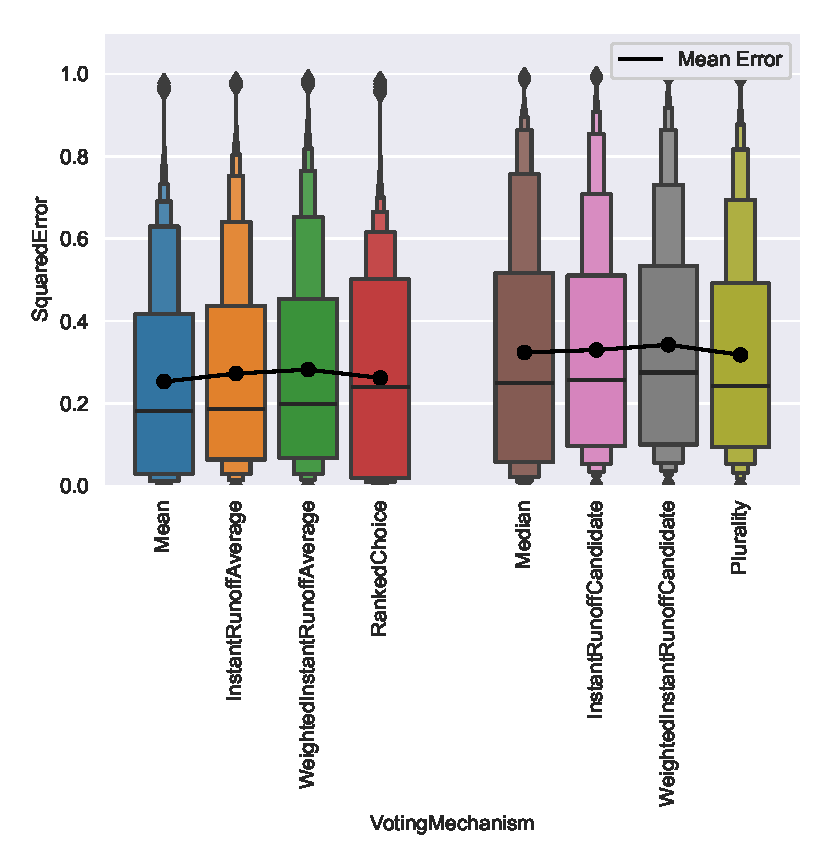
\includegraphics[scale=0.75]
    {./content/figures/voting_mechanisms/voting_mechanisms_comparison}
    \caption{Squared error populations by voting mechanism, with average
    mechanisms on the left and candidate mechanisms on the right.}
    \label{fig:voting-mechanisms-comparison}
\end{figure}

This graph immediately tells us a few things.
First, the squared error seems to be skewed, favoring numbers closer to 0.
This means there is a fairly even spread of estimates, since this is the
pattern one would expect to see from a uniform distribution of estimates.
Interestingly, however, is the majority of most error populations are
somewhere between a uniform distribution of estimates
(\autoref{fig:expected_even_distribution_squared_error}) and a normal
distribution (\autoref{fig:expected_gaussian_distribution_squared_error}).
Indeed, if the estimates are instead graphed as in
\autoref{fig:voting_mechanisms_estimate_distribution}, the distribution of estimates
is more normal than uniform.
This means most mechanisms are better at estimating \truth\ than random chance.

\begin{table}[htbp]
    % increase table row spacing, adjust to taste
    \renewcommand{\arraystretch}{1.0}

    \caption{The mean squared error for each mechanism, ordered lowest to highest.}
    \label{tab:voting-mechanism-mean-error}

    \centering
    \begin{tabular}{|c|c|}
        \hline
        Voting Mechanism                    & Mean Squared Error \\
        \hhline{|=|=|}
        Mean                                & 0.253191           \\
        \hline
        Ranked Choice                       & 0.262085           \\
        \hline
        Instant Runoff (Average)            & 0.272652           \\
        \hline
        Weighted Instant Runoff (Average)   & 0.282148           \\
        \hline
        Plurality                           & 0.318054           \\
        \hline
        Median                              & 0.323846           \\
        \hline
        Instant Runoff (Candidate)          & 0.329869           \\
        \hline
        Weighted Instant Runoff (Candidate) & 0.342495           \\
        \hline
    \end{tabular}
\end{table}

Additionally, while all distributions appear generally close, there appears to be a
slight difference between average and candidate mechanisms.
This can be confirmed by comparing the average mechanisms to the candidate mechanisms
using a Mann-Whitney U-test, with the alternative being the average mechanisms'
squared error is lesser.
Performing such a test results in a p-value of 0.0, far below the $\alpha$ of 0.05.
Since candidate mechanisms can still be useful depending on the situation, both the
best average mechanisms and the best candidate mechanisms will be identified.

Further U-tests were performed, comparing each individual voting mechanism against
every other individual mechanism.
The results of this analysis can be found in
\autoref{fig:all-voting-mechanisms-p-values}, and is further segmented and discussed in
\autoref{subsec:lowest-error-average-mechanisms} and
\autoref{subsec:lowest-error-candidate-mechanisms}.

\subsection{Average Mechanisms}\label{subsec:lowest-error-average-mechanisms}
Average mechanisms, as described in \autoref{subsubsec:average-mechanisms}, work by
averaging the estimates of the system's agents, so it is not too surprising they
result in less error than candidate mechanisms which ultimately output only a single
agent's estimate.
However, they are not all created equally.
This leads us to the question: which average mechanisms generally work best?

To start, an ANOVA test was performed on the average mechanisms.
This produced a p-value of 0, indicating there is very likely a difference between
average mechanisms.
U-tests were then performed to compare each mechanism on its own against each other
mechanism individually, resulting in \autoref{fig:average-mechanisms-p-values}.
The numbers next to the edges are the resultant p-values, where the alternative is
the population is lower than the other.
As is shown by the graph, there is sufficient evidence to reject the null hypothesis
than any of the populations are the same.

\begin{figure}[htbp]
    \centering
    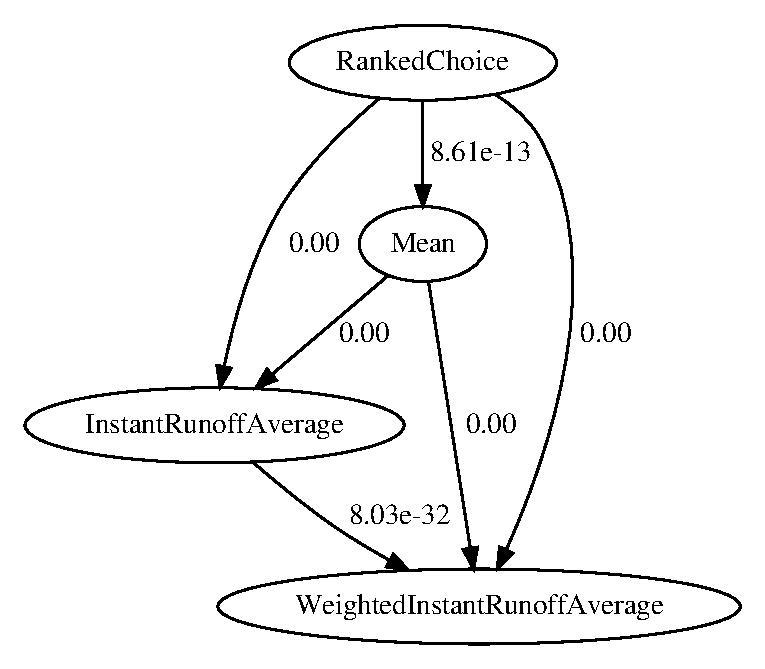
\includegraphics[scale=0.75]
    {./content/figures/voting_mechanisms/average-mechanisms-p-values.gv}
    \caption{The p-values for average voting mechanisms, given the alternative is one
    population is lesser than the other.
    An arrow pointing to another voting mechanism indicates the `from' mechanism
    beats the `to' mechanism.}
    \label{fig:average-mechanisms-p-values}
\end{figure}

In addition, Ranked Choice appears to beat out every other voting mechanism, followed
by Mean beating two, then Weight by Instant Runoff beating one, and finally Averaged
Weighted Instant Runoff beating none.
\begin{samepage}
    This means the rankings of the average mechanisms is as follows:
    \begin{enumerate}
        \item \hyperref[para:avg-ranked-choice]{Ranked Choice}
        \item \hyperref[para:mean]{Mean}
        \item \hyperref[para:avg-instant-runoff]{Weight by Instant Runoff}
        \item \hyperref[para:avg-weighted-instant-runoff]{Averaged Weighted Instant
        Runoff}
    \end{enumerate}
\end{samepage}

\subsection{Candidate Mechanisms}\label{subsec:lowest-error-candidate-mechanisms}
Candidate voting mechanisms are described in \autoref{subsubsec:candidate-mechanisms}.
They work by selecting a single `candidate' and uses its vote as \systemtruth.
While they do not appear to perform as well as average mechanisms, they may be
circumstances where they are required and so they will still be analyzed to determine
which candidate mechanism works best.

An ANOVA analysis was again used to start, which resulted in a p-value of
$2.49e-221$.
This, again, is clearly below $\alpha$, so we can reject the null hypothesis that all
populations are the same.
Following the pattern of analysis in
\autoref{subsec:lowest-error-average-mechanisms}, U-tests where then performed to
identify which mechanisms produced lower error than others.
The p-values can be found in \autoref{fig:candidate-mechanisms-p-values}.

\begin{figure}[htbp]
    \centering
    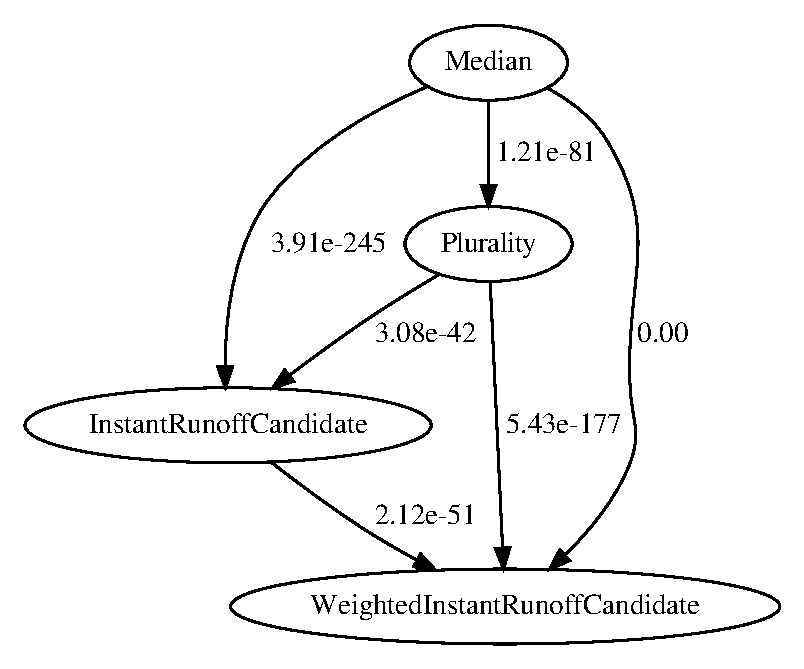
\includegraphics[scale=0.75]
    {./content/figures/voting_mechanisms/candidate-mechanisms-p-values.gv}
    \caption{The p-values for candidate voting mechanisms, given the alternative is one
    population is lesser than the other.
    An arrow pointing to another voting mechanism indicates the `from' mechanism
    beats the `to' mechanism.}
    \label{fig:candidate-mechanisms-p-values}
\end{figure}

While not as many p-values are 0 with the candidate mechanisms, there is still very
strong evidence that each candidate mechanism is not the same as each other.
For the candidate mechanisms, Median appears to be the best, followed
by Plurality, Instant Runoff, and finally Weighted Instant Runoff.
\begin{samepage}
    This means the rankings of the candidate mechanisms is as follows:
    \begin{enumerate}
        \item \hyperref[para:median]{Median}
        \item \hyperref[para:plurality]{Plurality}
        \item \hyperref[para:cand-instant-runoff]{Instant Runoff}
        \item \hyperref[para:cand-weighted-instant-runoff]{Weighted Instant Runoff}
    \end{enumerate}
\end{samepage}


\section{Lowest Error Weighting Mechanisms}\label{sec:lowest-error-weighting-mechanism}
Weighting mechanisms have a direct influence on how voting mechanisms operate in that
they apply weights to the estimates of the proxies.
This naturally has a direct impact on the output of a system.
\autoref{fig:weighting-mechanisms-comparison}

\begin{figure}[htbp]
    \centering
    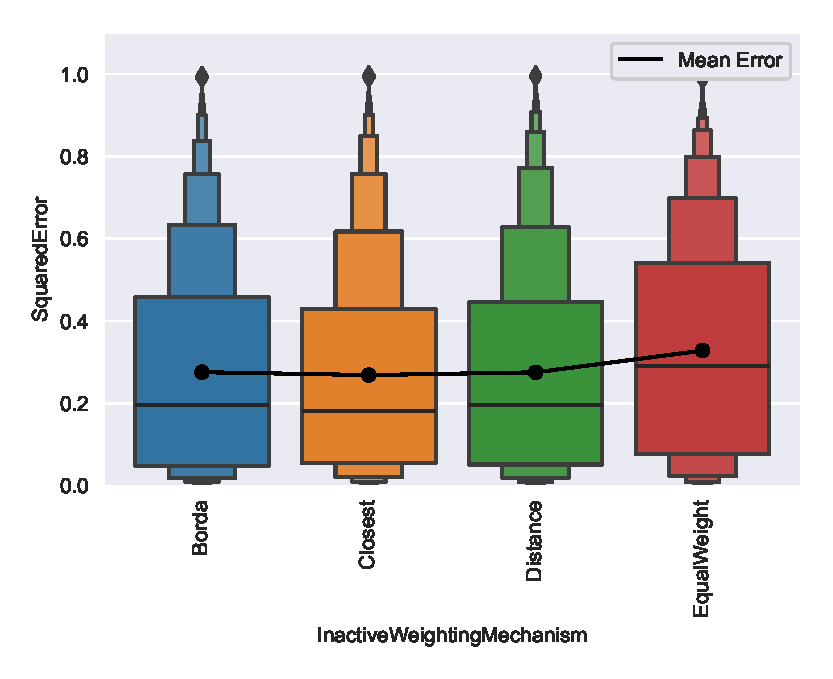
\includegraphics[scale=0.75]
    {./content/figures/weighting_mechanisms/weighting_mechanisms_comparison}
    \caption{Squared error populations by weighting mechanism.}
    \label{fig:weighting-mechanisms-comparison}
\end{figure}

\begin{table}[htbp]
    % increase table row spacing, adjust to taste
    \renewcommand{\arraystretch}{1.0}

    \caption{The mean squared error for each mechanism, ordered lowest to highest.}
    \label{tab:weighting-mechanism-mean-error}

    \centering
    \begin{tabular}{|c|c|}
        \hline
        Weighting Mechanism & Mean Squared Error \\
        \hhline{|=|=|}
        Closest             & 0.269045           \\
        \hline
        Distance            & 0.275722           \\
        \hline
        Borda               & 0.276065           \\
        \hline
        Equal Weight        & 0.328497           \\
        \hline
    \end{tabular}
\end{table}

While the mechanisms definitely appear close, there is a visible difference between
the Equal Weight mechanism and the other mechanisms.
This can be confirmed using a series of Mann-Whitney U-tests, resulting in
\autoref{fig:weighting-mechanisms-p-values}.
\begin{samepage}
    This gives us the ordering:
    \begin{enumerate}
        \item \hyperref[para:closest]{Vote for Closest}
        \item \hyperref[para:borda]{Borda}
        \item \hyperref[para:distance-voting]{Distance Voting}
        \item \hyperref[para:equal-weight]{Equal Weight}
    \end{enumerate}
\end{samepage}

\begin{figure}[htbp]
    \centering
    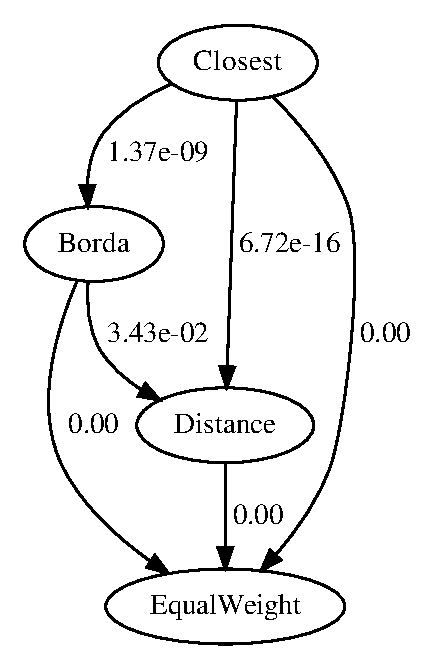
\includegraphics[scale=0.75]
    {./content/figures/weighting_mechanisms/weighting-mechanisms-p-values.gv}
    \caption{The p-values for weighting mechanisms, given the alternative is one
    population is lesser than the other.
    An arrow pointing to another voting mechanism indicates the `from' mechanism
    beats the `to' mechanism.}
    \label{fig:weighting-mechanisms-p-values}
\end{figure}

These results are somewhat surprising in that the simplest method, arguably barring
Equal Weight, appears to produce the best results.
This may be due to the Closest mechanism yielding a lower system-wide weight while
still maintaining an ordering of preferences.
However, this does not necessarily mean the Closest mechanism pairs best with all
voting mechanisms.
This idea is explored in~\fullref{sec:lowest-error-overall-combination}.


\section{Lowest Error Combination}\label{sec:lowest-error-overall-combination}
While the previous sections have explored the lowest error for each voting mechanism and
weighting mechanism regardless of the mechanism it's paired with, this section will
explore the lowest error for each combination of voting and weighting mechanism.

The population of error for each combination is displayed in
\autoref{fig:combined-comparison}, where we see a similar pattern with the voting
mechanisms as what was discussed in \autoref{sec:lowest-error-voting-mechanism}: the
candidate mechanisms tend to be noticeably worse than the average mechanisms.
Additionally, average mechanisms typically produce an error below the weighting
mechanism mean, while candidate mechanisms tend to produce an error that is higher
than the mean.

\begin{figure}[htbp]
    \centering
    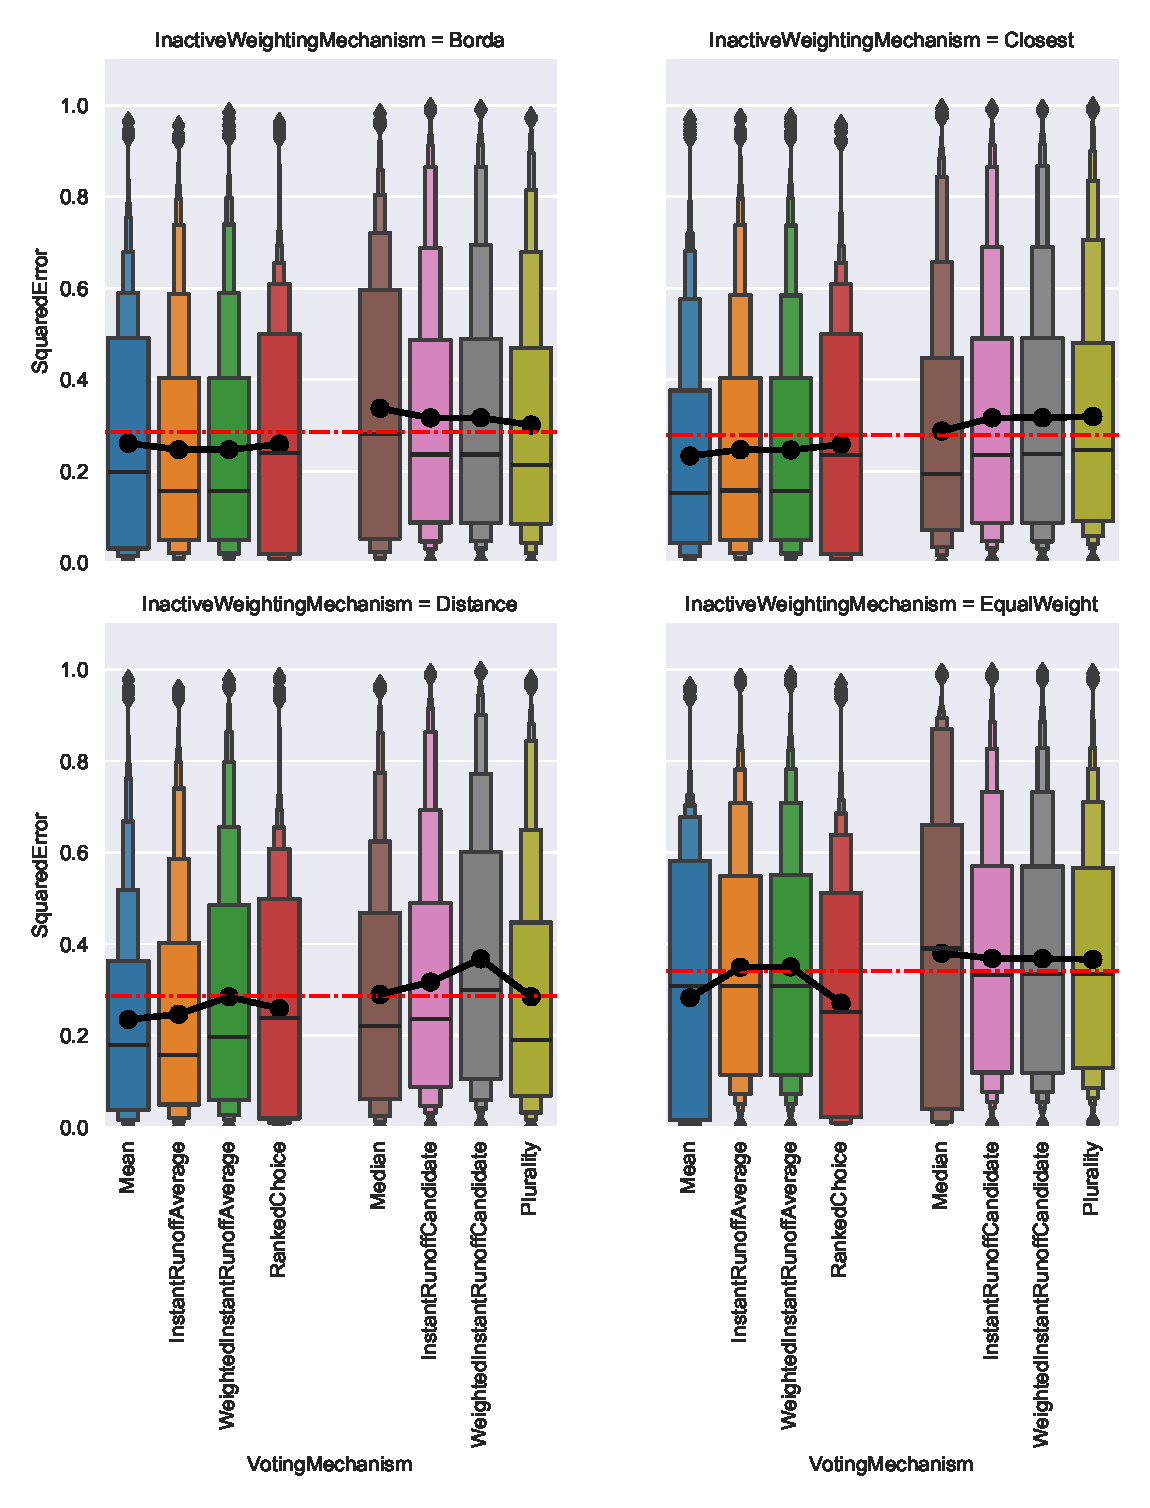
\includegraphics[scale=0.75]
    {./content/figures/combinations/combined_comparison}
    \caption{Squared error populations by combination of mechanisms. The red dashed
    line represents the mean for each weighting mechanism, while the black line with
    dots are the means for each voting mechanism using the weighting mechanism.}
    \label{fig:combined-comparison}
\end{figure}

Using U-tests, we can discover which combinations produce the lowest error.
By counting how many times some combination beats other combinations, we can produce
an over ranking.
The number of times one combination `beats' another by having a lower error is
displayed in \autoref{fig:combined-lesser_counts}, and is further tabulated in
\autoref{tab:combined-overall-rankings}.
From these tests, we can see the averaged easily dominate, with the first candidate
combination being in rank 15, reinforcing the idea that average mechanisms result in
lower error than candidate mechanisms.

\begin{figure}[htbp]
    \centering
    \includegraphics[scale=0.75]
    {./content/figures/combinations/combined_lesser_counts}
    \caption{The number of times each combination has a lower error according to
    U-tests.}
    \label{fig:combined-lesser_counts}
\end{figure}

From the graph, we can see our findings in~\fullref{sec:lowest-error-voting-mechanism}
hold true with the combinations as well, with Ranked Choice taking the top three ranks.
The rankings from~\fullref{sec:lowest-error-weighting-mechanism} also
generally hold true, since the Closest and Borda mechanisms generally
appear sooner than others.
It is possible, however, that voting mechanisms have a larger impact than weighting
mechanisms, since the general order of rankings more closely follows the voting
mechanism ordering rather than that of the weighting mechanisms.

%% I'm leaving this here in case I want to add it later. For now it seems like overkill
% Nevertheless, there may be occasions when candidate mechanisms may be preferable
% over average mechanisms, and so a deeper dive will be performed on both types of
% voting mechanisms.
%
% \subsection{Average Mechanisms}\label{subsec:lowest-error-combo-average}
%
% \subsection{Candidate Mechanisms}\label{subsec:lowest-error-combo-candidate}


\begin{table}[htbp]
    % increase table row spacing, adjust to taste
    \renewcommand{\arraystretch}{1.0}

    \caption{The rankings of combinations, ordered by the number of combinations
    beaten.
    The maximum number of combinations is 31 (32 total combinations, minus
    the combination being tested).
    Note that those with the same count are arranged in no particular order.}
    \label{tab:combined-overall-rankings}

    \centering
    \begin{tabular}{|c|c|c|}
        \hline
        Voting Mechanism                 & Weighting Mechanism & \# of Combos Beaten \\
        \hhline{|=|=|=|}
        Ranked Choice                    & Distance Voting     & 28                  \\
        \hline
        Ranked Choice                    & Closest             & 28                  \\
        \hline
        Ranked Choice                    & Borda               & 28                  \\
        \hline
        Mean                             & Closest             & 28                  \\
        \hline
        Mean                             & Distance Voting     & 27                  \\
        \hline
        Mean                             & Equal Weight        & 25                  \\
        \hline
        Ranked Choice                    & Equal Weight        & 24                  \\
        \hline
        Weight by Instant Runoff         & Borda               & 19                  \\
        \hline
        Averaged Weighted Instant Runoff & Borda               & 19                  \\
        \hline
        Weight by Instant Runoff         & Closest             & 19                  \\
        \hline
        Averaged Weighted Instant Runoff & Closest             & 19                  \\
        \hline
        Mean                             & Borda               & 19                  \\
        \hline
        Weight by Instant Runoff         & Distance Voting     & 19                  \\
        \hline
        Averaged Weighted Instant Runoff & Distance Voting     & 18                  \\
        \hline
        Plurality                        & Distance Voting     & 17                  \\
        \hline
        Median                           & Closest             & 16                  \\
        \hline
        Median                           & Distance Voting     & 15                  \\
        \hline
        Plurality                        & Borda               & 14                  \\
        \hline
        Weighted Instant Runoff          & Borda               & 8                   \\
        \hline
        Instant Runoff (Candidate)       & Distance Voting     & 8                   \\
        \hline
        Instant Runoff (Candidate)       & Closest             & 8                   \\
        \hline
        Instant Runoff (Candidate)       & Borda               & 8                   \\
        \hline
        Weighted Instant Runoff          & Closest             & 8                   \\
        \hline
        Median                           & Borda               & 8                   \\
        \hline
        Plurality                        & Closest             & 7                   \\
        \hline
        Median                           & Equal Weight        & 6                   \\
        \hline
        Averaged Weighted Instant Runoff & Equal Weight        & 4                   \\
        \hline
        Weight by Instant Runoff         & Equal Weight        & 4                   \\
        \hline
        Weighted Instant Runoff          & Distance Voting     & 3                   \\
        \hline
        Instant Runoff (Candidate)       & Equal Weight        & 1                   \\
        \hline
        Weighted Instant Runoff          & Equal Weight        & 1                   \\
        \hline
        Plurality                        & Equal Weight        & 0                   \\
        \hline
    \end{tabular}
\end{table}


\section{Weightlessly Averaging All Agents}\label{sec:weightless-average-all}
% Explain how WeightlessAverageAll works best
While the results thus far have been very interesting, the question of if using such
systems works better than simply averaging the estimates of all agents.
Such an operation is here dubbed `weightlessly averaging all,' since it ignores
weights and simply averages all agents, including inactive agents.
This technique does not use a weighting mechanism.
\autoref{fig:weightless-voting-mechanisms-comparison} shows how weightlessly
averaging all agents compares to the other mechanisms, ignoring which weighting
mechanism is used or the distribution of the proxies or inactive agents.

\begin{figure}[htbp]
    \centering
    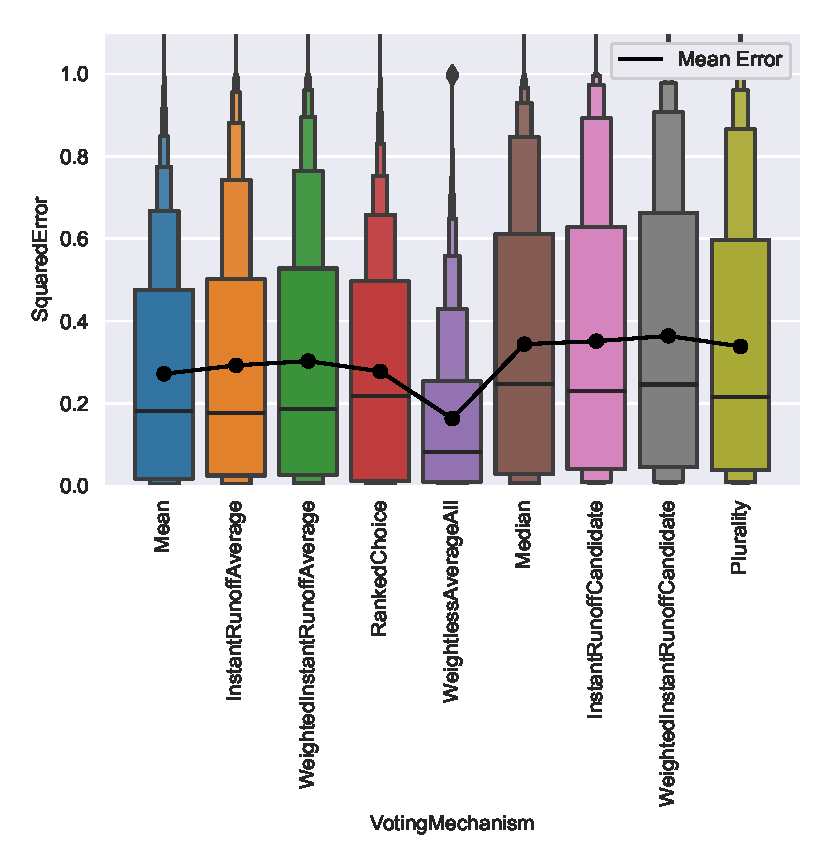
\includegraphics[scale=0.75]
    {./content/figures/weightless/weightless_voting_mechanisms_comparison}
    \caption{Squared error populations by voting mechanism, with average
    mechanisms on the left and candidate mechanisms on the right.
    Weightlessly averaging all agents' estimates is in the center.}
    \label{fig:weightless-voting-mechanisms-comparison}
\end{figure}

It is immediately evident that weightlessly averaging all agents' estimates works
considerable better that using proxy vote systems.
While this would initially indicate that proxy vote systems should not be used when a
simpler and more accurate technique already exists, this broad overview does not tell
the full story.
As explored previously, each voting mechanism is also paired with a weighting
mechanism that heavily influences its accuracy.
Additionally, we have yet to explore how the proxy and inactive estimate
distributions interact with the different mechanisms.

Indeed, performing tests on group separated by voting and weighting mechanisms as
well as proxy and inactive estimate distribution, indicates 467 of the 2048 possible
combinations, or 22.80\%, work better using a proxy vote system than weightlessly
averaging.
These tests are performed as if the proxy system was used instead of weightlessly
averaging, meaning that if the tests are performed groups with the same proxy and
inactive estimate distributions.

Of these 467 combinations, 223 (47.75\%) have an asymmetric proxy distribution with
a symmetric inactive distribution, while 154 (32.98\%) have an asymmetric inactive
distribution with a symmetric inactive distribution.
Additionally, 78 (16.70\%) use asymmetric distributions for both proxies and
inactive agents.
This totals to 455 (97.43\%) of the 467 more accurate proxy systems that use
asymmetric distributions!

The remaining 12 consist of high-performing voting mechanism/weighting mechanism
combinations, as discovered in \autoref{sec:lowest-error-overall-combination},
using Gaussian or \betadistribution{4}{4} distributions for the proxies,
and \betadistribution{0.3}{0.3} as the inactive distributions.
These combinations are displayed in~\autoref{tab:non-asymmetric-lower-pop-systems}.

\begin{table}[htbp]
    % increase table row spacing, adjust to taste
    \renewcommand{\arraystretch}{1.0}

    \caption{The proxy voting systems that still achieve a lower error than
    weightless average all, in no particular order.}
    \label{tab:non-asymmetric-lower-pop-systems}

    \centering
    \begin{tabular}{|c|c|c|c|}
        \hline
        Voting Mechanism & %
        Weighting Mechanism & %
        Proxy Distribution & %
        Inactive Distribution \\
        \hhline{|=|=|=|=|}
        Mean & Borda & \betadistribution{4}{4} & \betadistribution{0
        .3}{0.3} \\
        \hline
        Mean & Equal Weight & \betadistribution{4}{4} & \betadistribution{0
        .3}{0.3} \\
        \hline
        Mean & Borda & Gaussian & \betadistribution{0
        .3}{0.3} \\
        \hline
        Mean & Distance & Gaussian & \betadistribution{0
        .3}{0.3} \\
        \hline
        Mean & Equal Weight & Gaussian & \betadistribution{0
        .3}{0.3} \\
        \hline
        Ranked Choice & Borda & \betadistribution{4}{4} & \betadistribution{0
        .3}{0.3} \\
        \hline
        Ranked Choice & Closest & \betadistribution{4}{4} & \betadistribution{0
        .3}{0.3} \\
        \hline
        Ranked Choice & Distance & \betadistribution{4}{4} & \betadistribution{0
        .3}{0.3} \\
        \hline
        Ranked Choice & Borda & Gaussian & \betadistribution{0
        .3}{0.3} \\
        \hline
        Ranked Choice & Closest & Gaussian & \betadistribution{0
        .3}{0.3} \\
        \hline
        Ranked Choice & Distance & Gaussian & \betadistribution{0
        .3}{0.3} \\
        \hline
        Ranked Choice & Equal Weight & Gaussian & \betadistribution{0
        .3}{0.3} \\
        \hline
    \end{tabular}
\end{table}

However, this does not mean a proxy system is always better when some distribution is
asymmetrical.
The number of lower error asymmetric combinations is only 29.62\% of the 1536
possible combinations with at least one distribution asymmetric, and all 467 lower error
combinations are only 22.80\% of all 2048 combinations.
Ten combinations with at least one asymmetric distribution failed to achieve a lower
error, regardless of the mechanism used.
These combinations are shown in \autoref{tab:no-appearance-distro-combos}.
Of note is in all these combinations, both distributions are asymmetric.
Additionally, whenever an asymmetric distribution is placed with itself, a proxy system
does not produce a lower error.
Finally, the more heavily skewed asymmetric distributions work worse with other
asymmetric distributions.

\begin{table}[htbp]
    % increase table row spacing, adjust to taste
    \renewcommand{\arraystretch}{1.0}

    \caption{The asymmetric distribution combinations that were never found to achieve
    lower error than weightlessly averaging, arranged in no particular order.}
    \label{tab:no-appearance-distro-combos}

    \centering
    \begin{tabular}{|c|c|}
        \hline
        Proxy Distribution        & Inactive Distribution     \\
        \hhline{|=|=|}
        \betadistribution{0.3}{3} & \betadistribution{0.3}{3} \\
        \hline
        \betadistribution{0.3}{3} & \betadistribution{3}{0.3} \\
        \hline
        \betadistribution{0.3}{3} & \betadistribution{4}{1}   \\
        \hline
        \betadistribution{1}{4}   & \betadistribution{1}{4}   \\
        \hline
        \betadistribution{1}{4}   & \betadistribution{4}{1}   \\
        \hline
        \betadistribution{3}{0.3} & \betadistribution{0.3}{3} \\
        \hline
        \betadistribution{3}{0.3} & \betadistribution{1}{4}   \\
        \hline
        \betadistribution{3}{0.3} & \betadistribution{3}{0.3} \\
        \hline
        \betadistribution{4}{1}   & \betadistribution{1}{4}   \\
        \hline
        \betadistribution{4}{1}   & \betadistribution{4}{1}   \\
        \hline
    \end{tabular}
\end{table}

A natural next question is which mechanism combinations are more likely to produce a
lower error?
The count of how many times each voting mechanism/weighting mechanism combination
tests to have a lower error than weightlessly averaging in displayed
in~\autoref{tab:lower-pop-combo-count}.
This table would seem to indicate that the stronger combinations are more able to
achieve a lower error.
Surprisingly, even candidate mechanisms are occasionally able to achieve a lower error
as well.

\begin{table}[htbp]
    % increase table row spacing, adjust to taste
    \renewcommand{\arraystretch}{1.0}

    \caption{The count of mechanism combinations the achieve a lower error
    population than weightlessly averaging, ordered by count, then voting mechanism,
        and finally weighting mechanism.}
    \label{tab:lower-pop-combo-count}

    \centering
    \begin{tabular}{|c|c|c|}
        \hline
        Voting Mechanism                    & Weighting Mechanism & Count \\
        \hhline{|=|=|=|}
        Mean                                & Equal Weight        & 20    \\
        \hline
        Plurality                           & Closest             & 20    \\
        \hline
        Ranked Choice                       & Borda               & 20    \\
        \hline
        Ranked Choice                       & Closest             & 20    \\
        \hline
        Ranked Choice                       & Distance            & 20    \\
        \hline
        Ranked Choice                       & Equal Weight        & 19    \\
        \hline
        Instant Runoff (Average)            & Borda               & 16    \\
        \hline
        Instant Runoff (Average)            & Closest             & 16    \\
        \hline
        Instant Runoff (Average)            & Distance            & 16    \\
        \hline
        Mean                                & Borda               & 16    \\
        \hline
        Mean                                & Closest             & 16    \\
        \hline
        Median                              & Closest             & 16    \\
        \hline
        Weighted Instant Runoff (Average)   & Borda               & 16    \\
        \hline
        Weighted Instant Runoff (Average)   & Closest             & 16    \\
        \hline
        Instant Runoff (Average)            & Equal Weight        & 14    \\
        \hline
        Instant Runoff (Candidate)          & Borda               & 14    \\
        \hline
        Instant Runoff (Candidate)          & Closest             & 14    \\
        \hline
        Instant Runoff (Candidate)          & Distance            & 14    \\
        \hline
        Median                              & Equal Weight        & 14    \\
        \hline
        Plurality                           & Distance            & 14    \\
        \hline
        Weighted Instant Runoff (Average)   & Equal Weight        & 14    \\
        \hline
        Weighted Instant Runoff (Candidate) & Borda               & 14    \\
        \hline
        Weighted Instant Runoff (Candidate) & Closest             & 14    \\
        \hline
        Instant Runoff (Candidate)          & Equal Weight        & 13    \\
        \hline
        Weighted Instant Runoff (Candidate) & Equal Weight        & 13    \\
        \hline
        Mean                                & Distance            & 11    \\
        \hline
        Plurality                           & Equal Weight        & 11    \\
        \hline
        Median                              & Borda               & 10    \\
        \hline
        Weighted Instant Runoff (Average)   & Distance            & 10    \\
        \hline
        Weighted Instant Runoff (Candidate) & Distance            & 10    \\
        \hline
        Median                              & Distance            & 8     \\
        \hline
        Plurality                           & Borda               & 8     \\
        \hline
    \end{tabular}
\end{table}

While it is clear that simply weightlessly averaging all agent's estimates is a more
accurate method, there appear to be occasions when proxy vote systems can reduce
error, particularly when one of the error distributions is asymmetrical.
This look into distributions and other parameters begs for a closer look and may yield
fascinating results upon closer inspection.


\section{How many Agents to Use}\label{sec:how-many-agents}
Regardless of which combination of mechanisms is used, the question still remains,
`How many proxies and inactive agents should be used?'
This question directly affects the cost of a system, since the cost is tied to the
number of agents, and so ideally the number of agents should be minimized.

There are three parts to this question, all of which will be addressed here.
The first is how many proxies should be used.
\autoref{fig:proxy-count} shows how proxy count affects the error of a system.
From this graph, we can see in the beginning more proxies produces better results.
However, this benefit reduces over time and eventually flattens out or, in the case
of some combinations, increases the error of a system.
This benefit seems to bottom out between 10 and 15 proxies.

\begin{figure}[htbp]
    \centering
    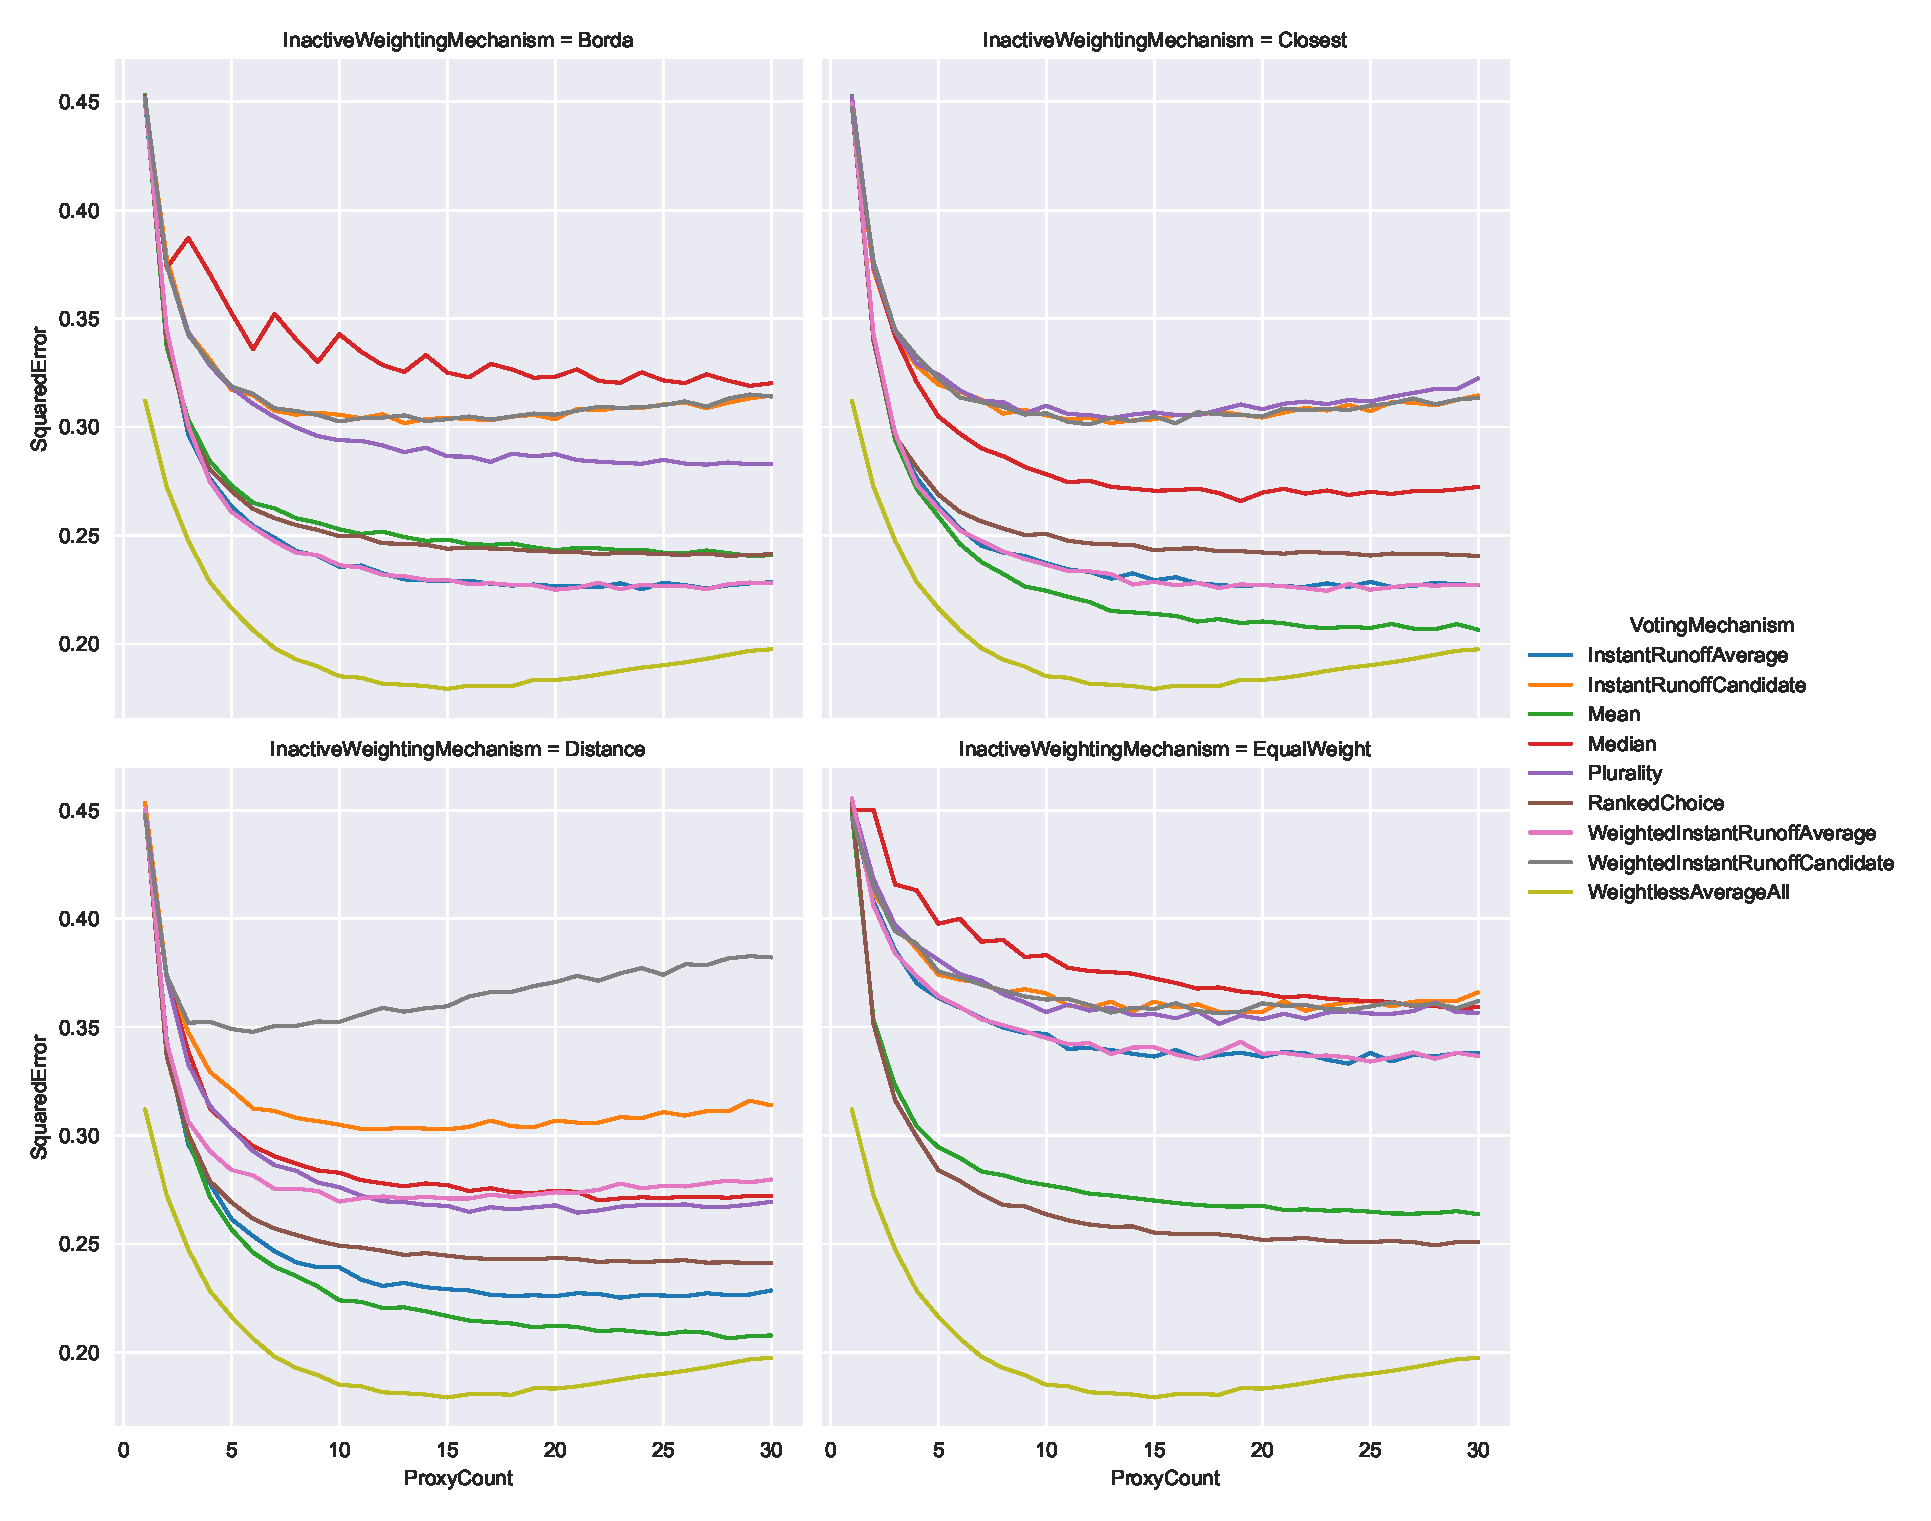
\includegraphics[
        width=\textwidth,
        height=\dimexpr
        \textheight - 4 % Could also be .9\textheight
        \baselineskip,
        keepaspectratio]
    {./content/figures/ratios/proxy_count}
    \caption{How the number of proxies affects the system error.}
    \label{fig:proxy-count}
\end{figure}

The second part of determining how many agents to use is how many inactive agents to
use.
As with minimizing the number of proxies, minimizing the number of inactive agents to
use will help reduce the costs of the system.
\autoref{fig:inactive-count} seems to indicate that, with the exception of
weightlessly averaging all agents, there is little benefit in using more inactive
agents.
This doesn't mean only one inactive agent should be used, as is indicated by the
third part of the question: the ratio between proxies and inactive agents.

\begin{figure}[htbp]
    \centering
    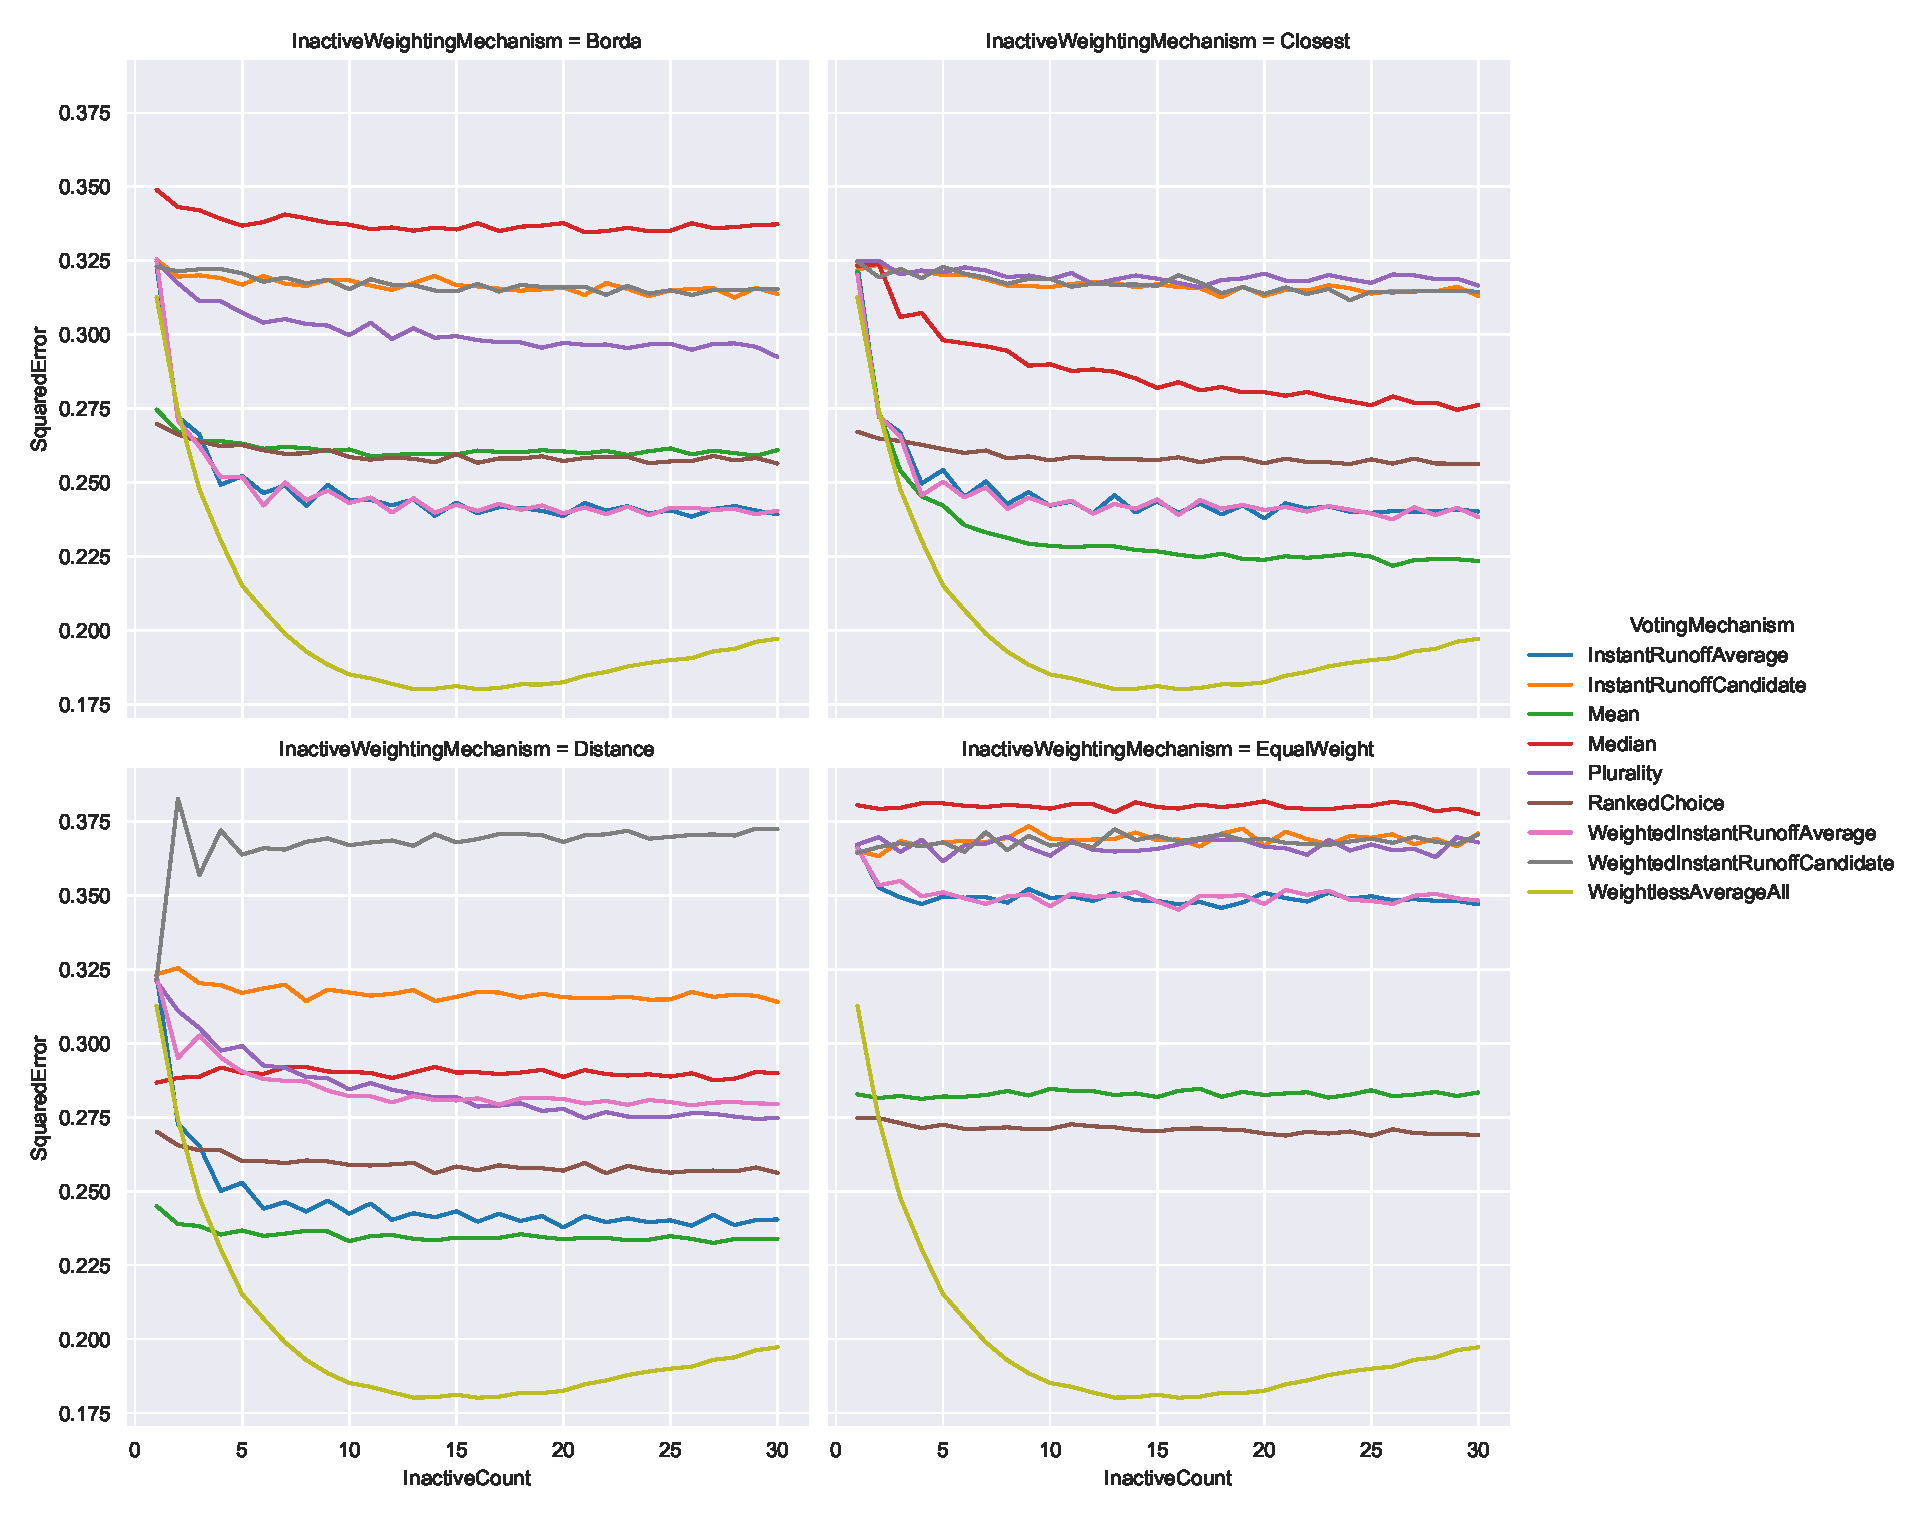
\includegraphics[
        width=\textwidth,
        height=\dimexpr
        \textheight - 4 % Could also be .9\textheight
        \baselineskip,
        keepaspectratio]
    {./content/figures/ratios/inactive_count}
    \caption{How the number of inactive agents affects the system error.}
    \label{fig:inactive-count}
\end{figure}

\autoref{fig:ratios}~and~\ref{fig:ratios-zoomed} display the error in the system as
the ratio between proxies and inactive agents increases, with
\autoref{fig:ratios-zoomed} providing a zoomed-in perspective.
Interestingly, the curve produced in each of these graphs flattens around a 1:1
ratio, indicating that there is little or no benefit to having a differing number of
proxies and inactive agents.
Additionally, there seems to be small `hiccups' at each whole number.
While the reason for this is not explored in this study, this would indicate that
slightly higher or lower ratio than 1:1 should be used.
With this mind, and since the number of inactive agents generally does not have an
effect on the system error, it would likely be best to use slightly fewer inactive
agents than proxy agents in an effort to decrease the total system cost and increase
system accuracy.

\begin{figure}[htbp]
    \centering
    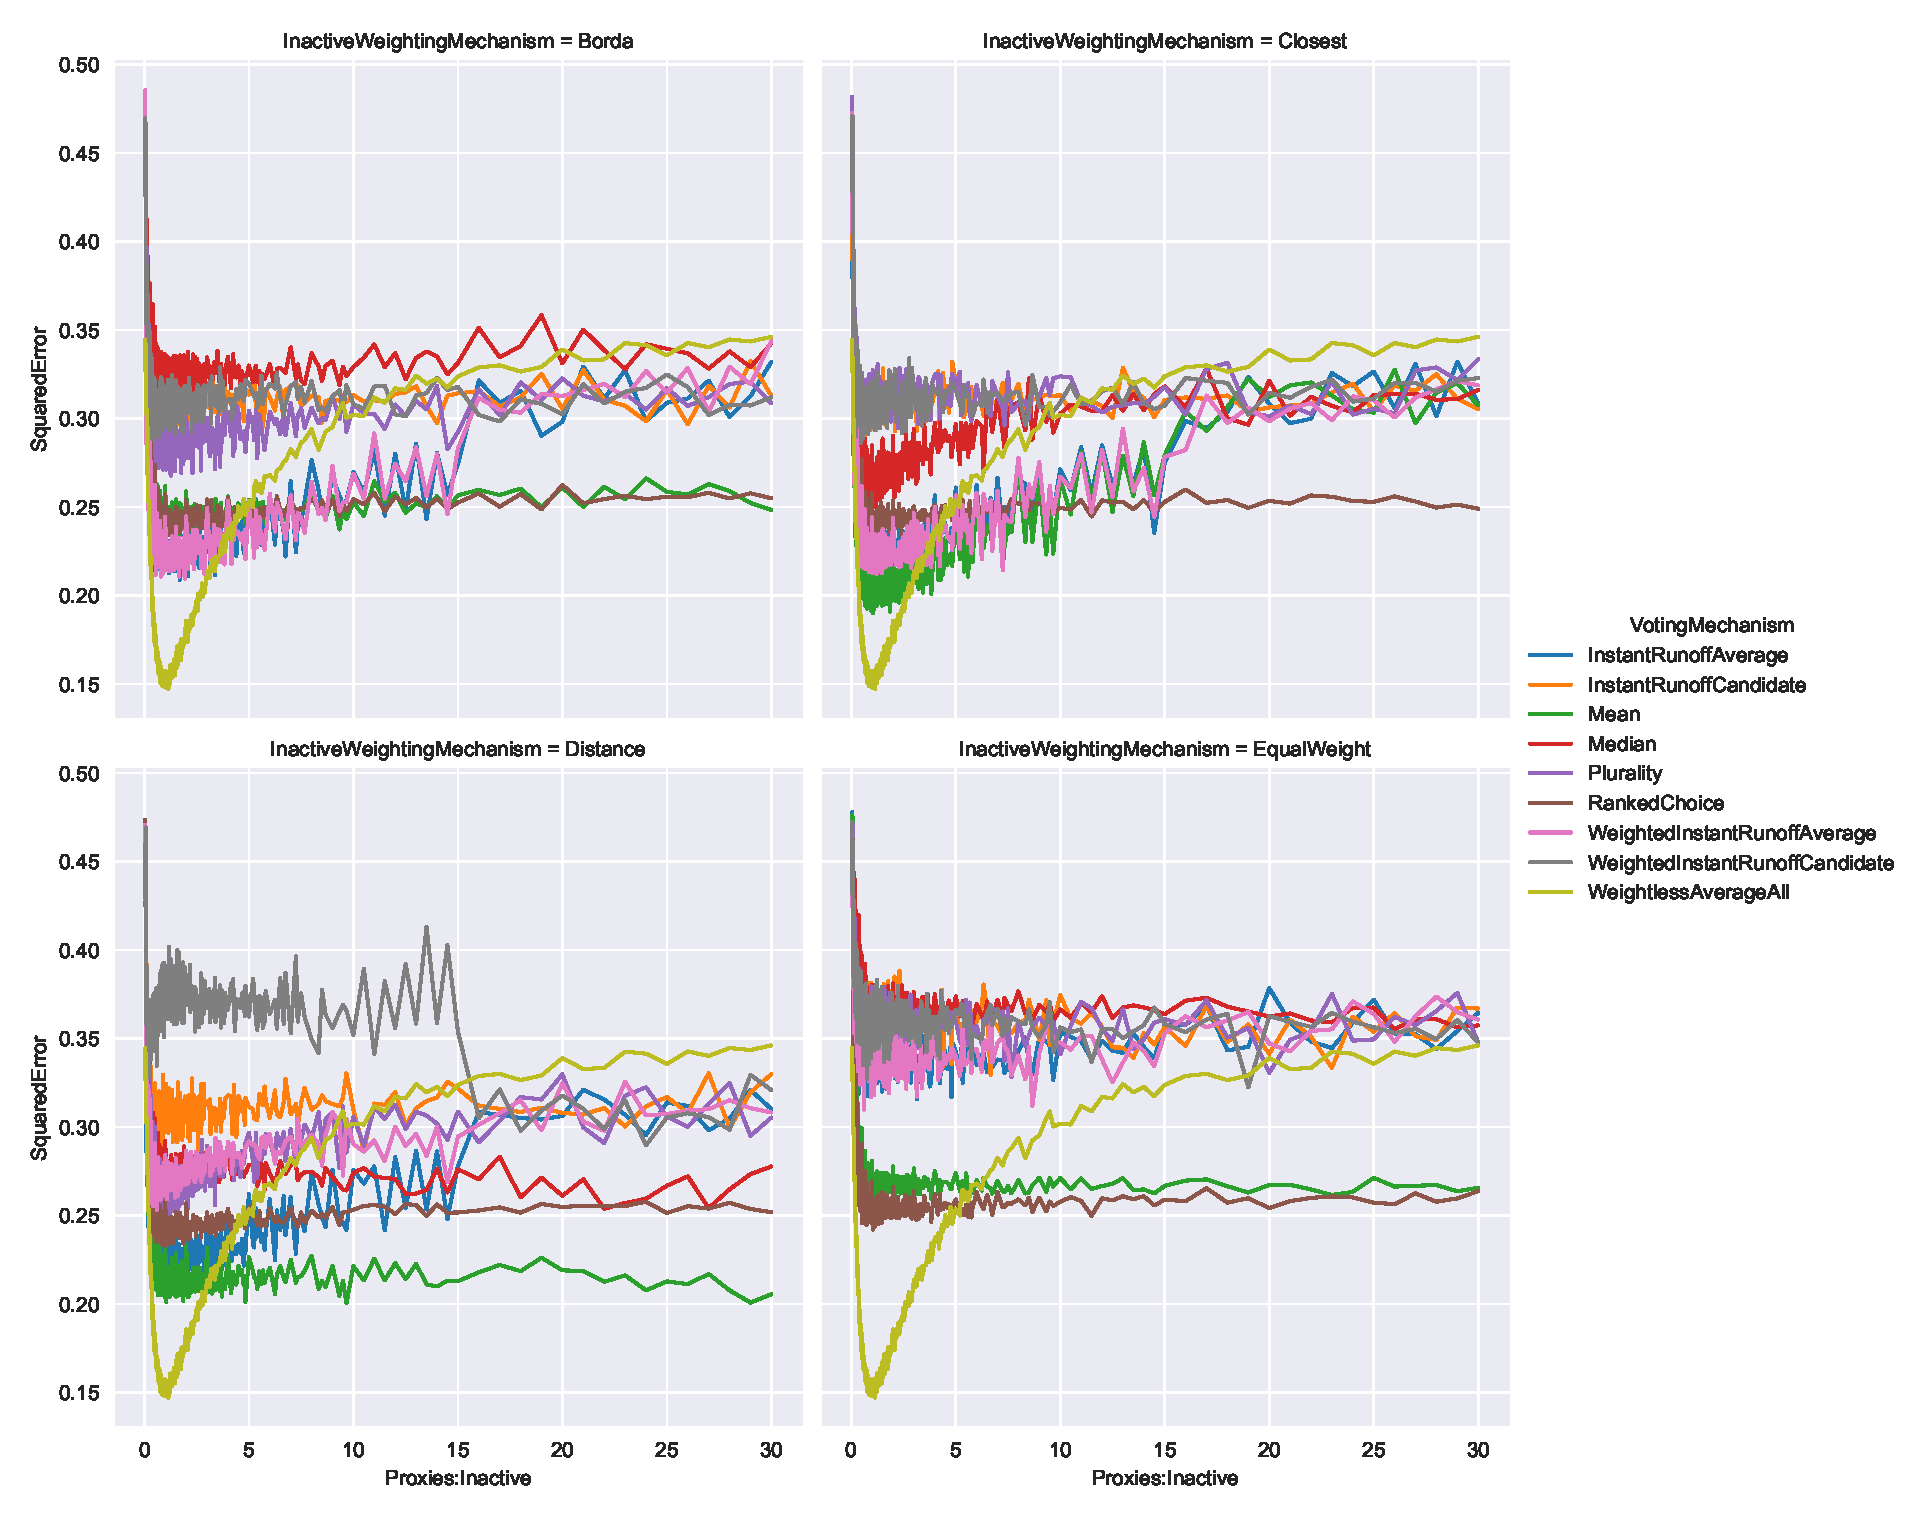
\includegraphics[
        width=\textwidth,
        height=\dimexpr
        \textheight - 4 % Could also be .9\textheight
        \baselineskip,
        keepaspectratio]
    {./content/figures/ratios/ratios}
    \caption{How the ratio between proxies and inactive agents affects the system
    error.}
    \label{fig:ratios}
\end{figure}

\begin{figure}[htbp]
    \centering
    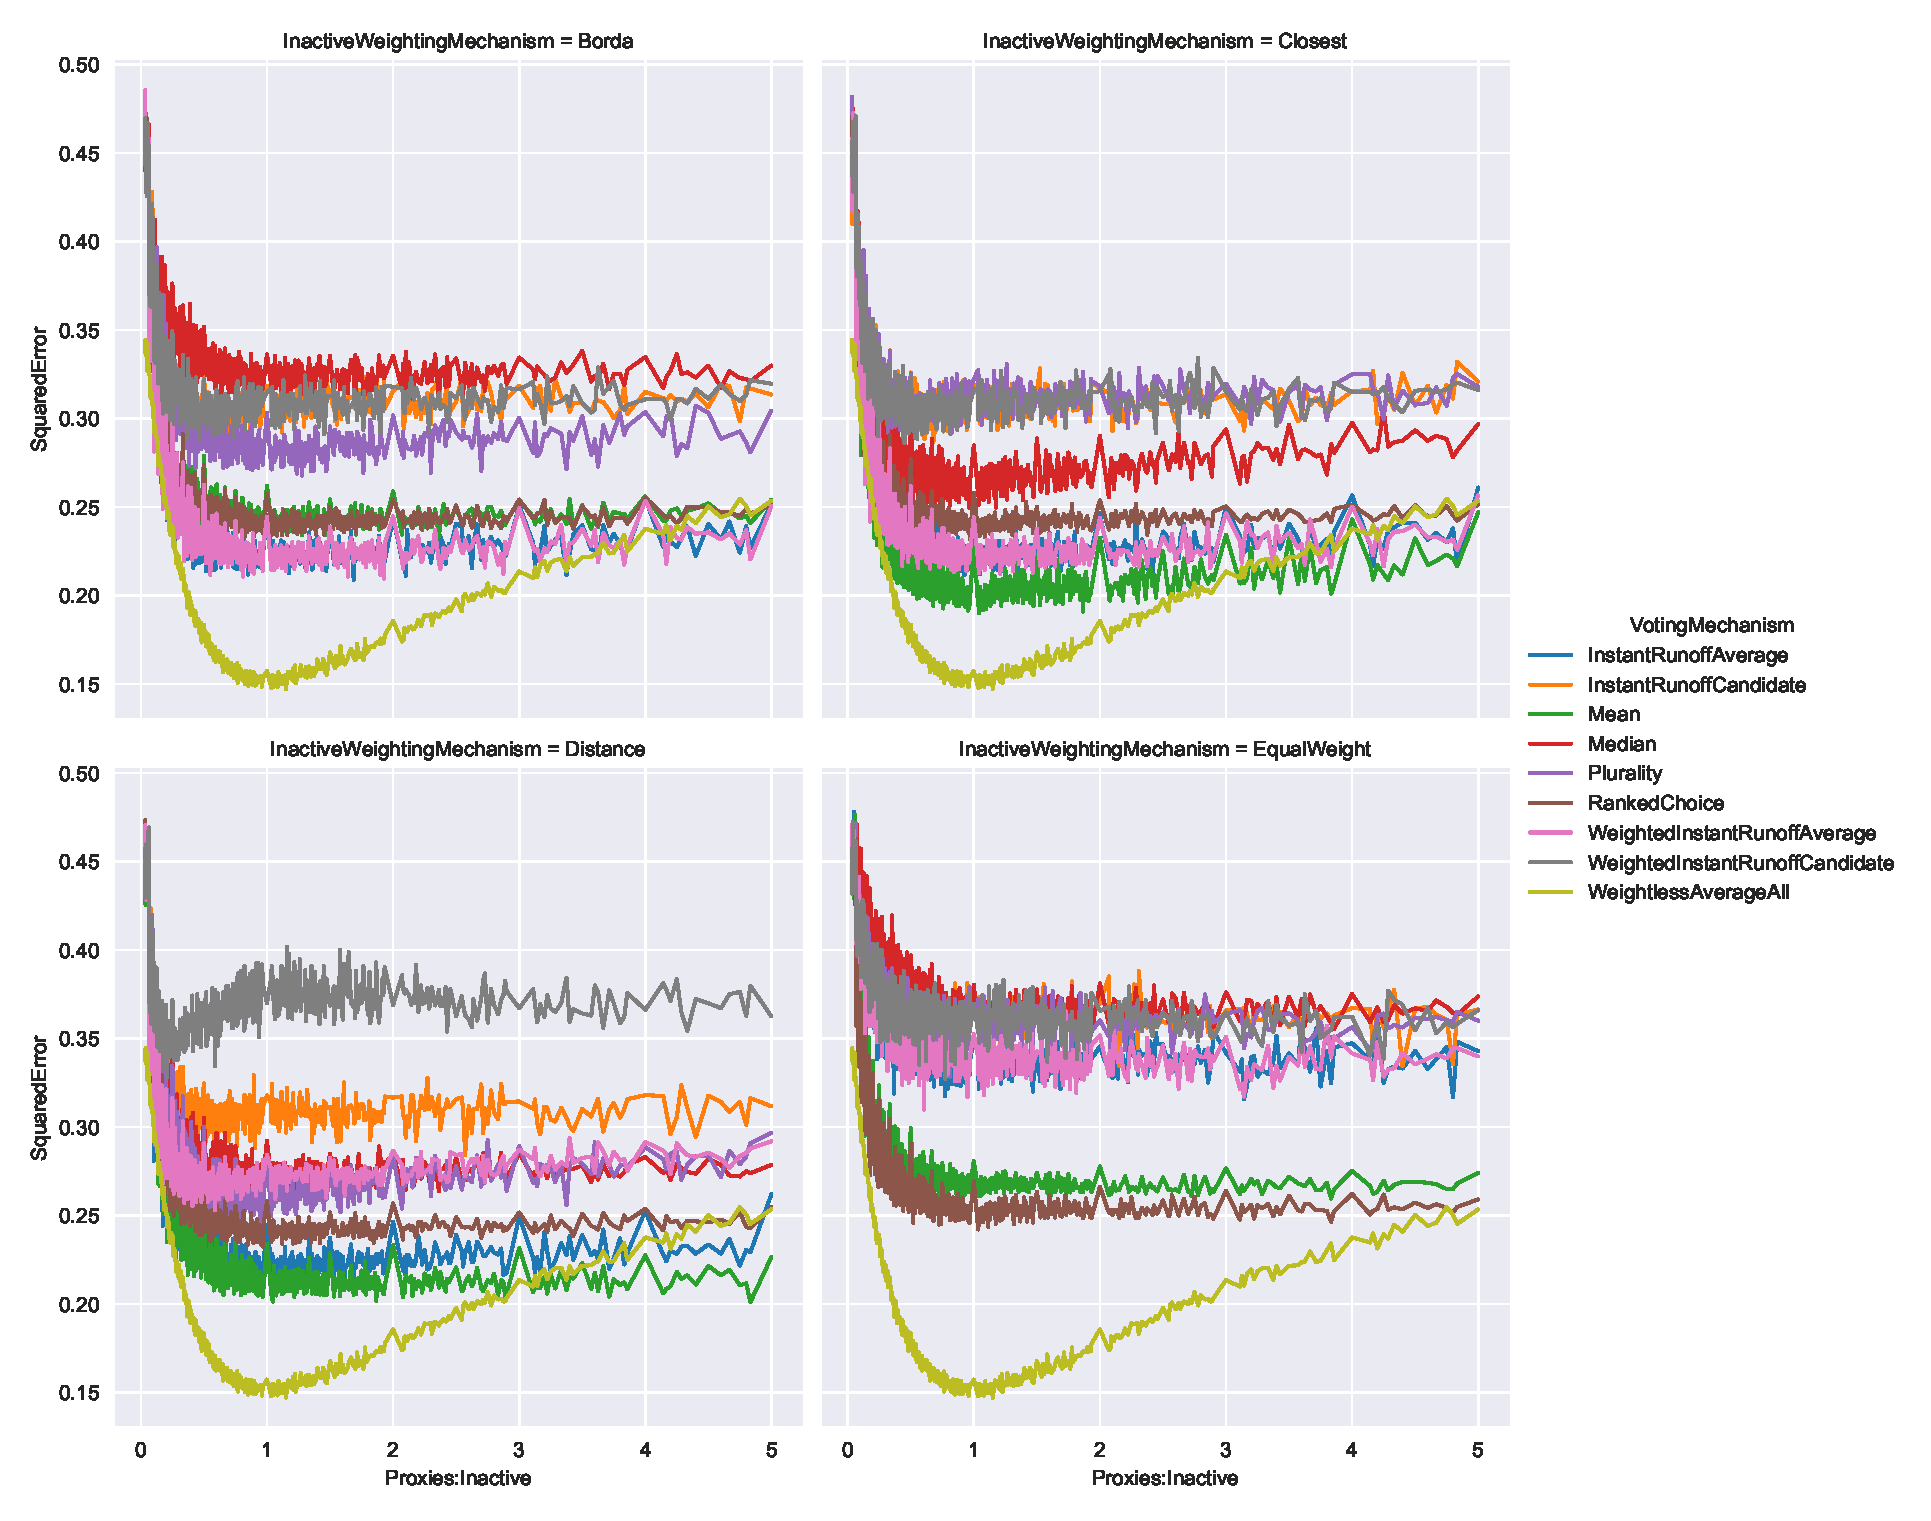
\includegraphics[
        width=\textwidth,
        height=\dimexpr
        \textheight - 4 % Could also be .9\textheight
        \baselineskip,
        keepaspectratio]
    {./content/figures/ratios/ratios_zoomed}
    \caption{How the ratio between proxies and inactive agents affects the system
    error. Zoomed in to better see the curve.}
    \label{fig:ratios-zoomed}
\end{figure}

    %
%  This is an example of how a LaTeX thesis should be formatted.  This
%  document contains chapter 2 of the thesis.
%
%  Time-stamp: "[sample-chapter2.tex] last modified by Scott Budge (scott) on 2016-07-28 (Thursday, 28 July 2016) at 08:40:50 on goga.ece.usu.edu"
%
%  Info: $Id: sample-chapter2.tex 967 2016-07-28 15:33:29Z scott $   USU
%  Revision: $Rev: 967 $
% $LastChangedDate: 2016-07-28 09:33:29 -0600 (Thu, 28 Jul 2016) $
% $LastChangedBy: scott $
%

\chapter{CONCLUSIONS AND FURTHER WORK}\label{ch:conclusions-and-further-work}

\section{Summary}\label{sec:summary}


\section{Further Work and Improvements}\label{sec:further-work-and-improvements}
% FIXME: This might need to be moved to Chapter 4
% - Multiple levels of expertise. Expert voters could have varying levels of
% accuracy, allowing for more complex systems.
% - (If I decide to restrict experts and untrained to the same mins and maxes)
% Allow for untrained to have a lower restriction, making them less accurate.
% - Independently track time, monetary cost, etc. for system cost (described
% in the cost section of Criteria. Useful identifying multiple systems for
% different costs.
% Closer look into instances where proxy voting works better than weightlessly averaging


    % Endmatter
    % For BibTeX references: specify a .bib file and a style.
    % The style used here is for IEEE transactions formatting:
    \references{
        references/IEEEabrv,
        references/research}
    {IEEEtran}

    % The style used here is for AIAA formatting:
%    \references{IEEEabrv,sample}{aiaa}

    %
%  Example Appendix pages.
%  Modified to use new usu-thesis-mk2 appendix facilities.
%
%  Time-stamp: "[appendix.tex] last modified by Scott Budge (scott) on
%  2021-06-28 (Monday, 28 June 2021) at 09:03:44 on goga.ece.usu.edu"
%
%  Info: $Id: appendix.tex 1183 2021-06-28 16:49:30Z scott $   USU
%  Revision: $Rev: 1183 $
% $LastChangedDate: 2021-06-28 10:49:30 -0600 (Mon, 28 Jun 2021) $
% $LastChangedBy: scott $
%
%
% For a single appendix, use \makeappendix, and place the 
% body of the appendix after it

%\makeappendix

% < single appendix body here >

% For multiple appendices, use \makeappendices, and create each appendix
% using \appendix{}
% For sub-appendices use \appendixsection{} and \appendixsubsection{}

\makeappendices
\appendix{Voting Distributions}\label{chap:voting-distributions}

\appendixsection{Percent inside Extents}
% TODO: Add description of table
This is placeholder text to ensure
\autoref{tab:distributions-percent-inside-extents} stays in the correct
location. % FIXME

% - Distribution of votes
%     - Uniform
%     - Gaussian
%     - Bimodal about center
%     - Skewed?

\begin{table}[htbp]
    % increase table row spacing, adjust to taste
    \renewcommand{\arraystretch}{1.3}

    \caption{List of distributions used by agents to vote.}
    \label{tab:distributions-percent-inside-extents}

    \centering
    \begin{tabular}{|c|c|c|}
        \hline
        Distribution      & Notation      & Percent inside Extents \\
        \hline
        Uniform           & \uniformdist  & 100\%                  \\
        \hline
        Normal (Gaussian) & \gaussiandist & 99.7\%                 \\
        \hline
        Beta              & \betadist     & 100\%                  \\
        \hline
    \end{tabular}
\end{table}

\appendixsection{Distributions used}
% TODO: Add graphs of distributions used
\begin{table}[htbp]
    % increase table row spacing, adjust to taste
    \renewcommand{\arraystretch}{1.3}

    \caption{List of distributions used by agents to vote.}
    \label{tab:distributions}

    \centering
    \begin{tabular}{|c|c|c|}
    \end{tabular}
\end{table}

\appendixsection{Distributions of Error}
The distribution of square error for each voting mechanism is displayed as a
KDE graph in \autoref{fig:voting_mechanisms_distribution}.

\begin{figure}[!t]
    \centering
    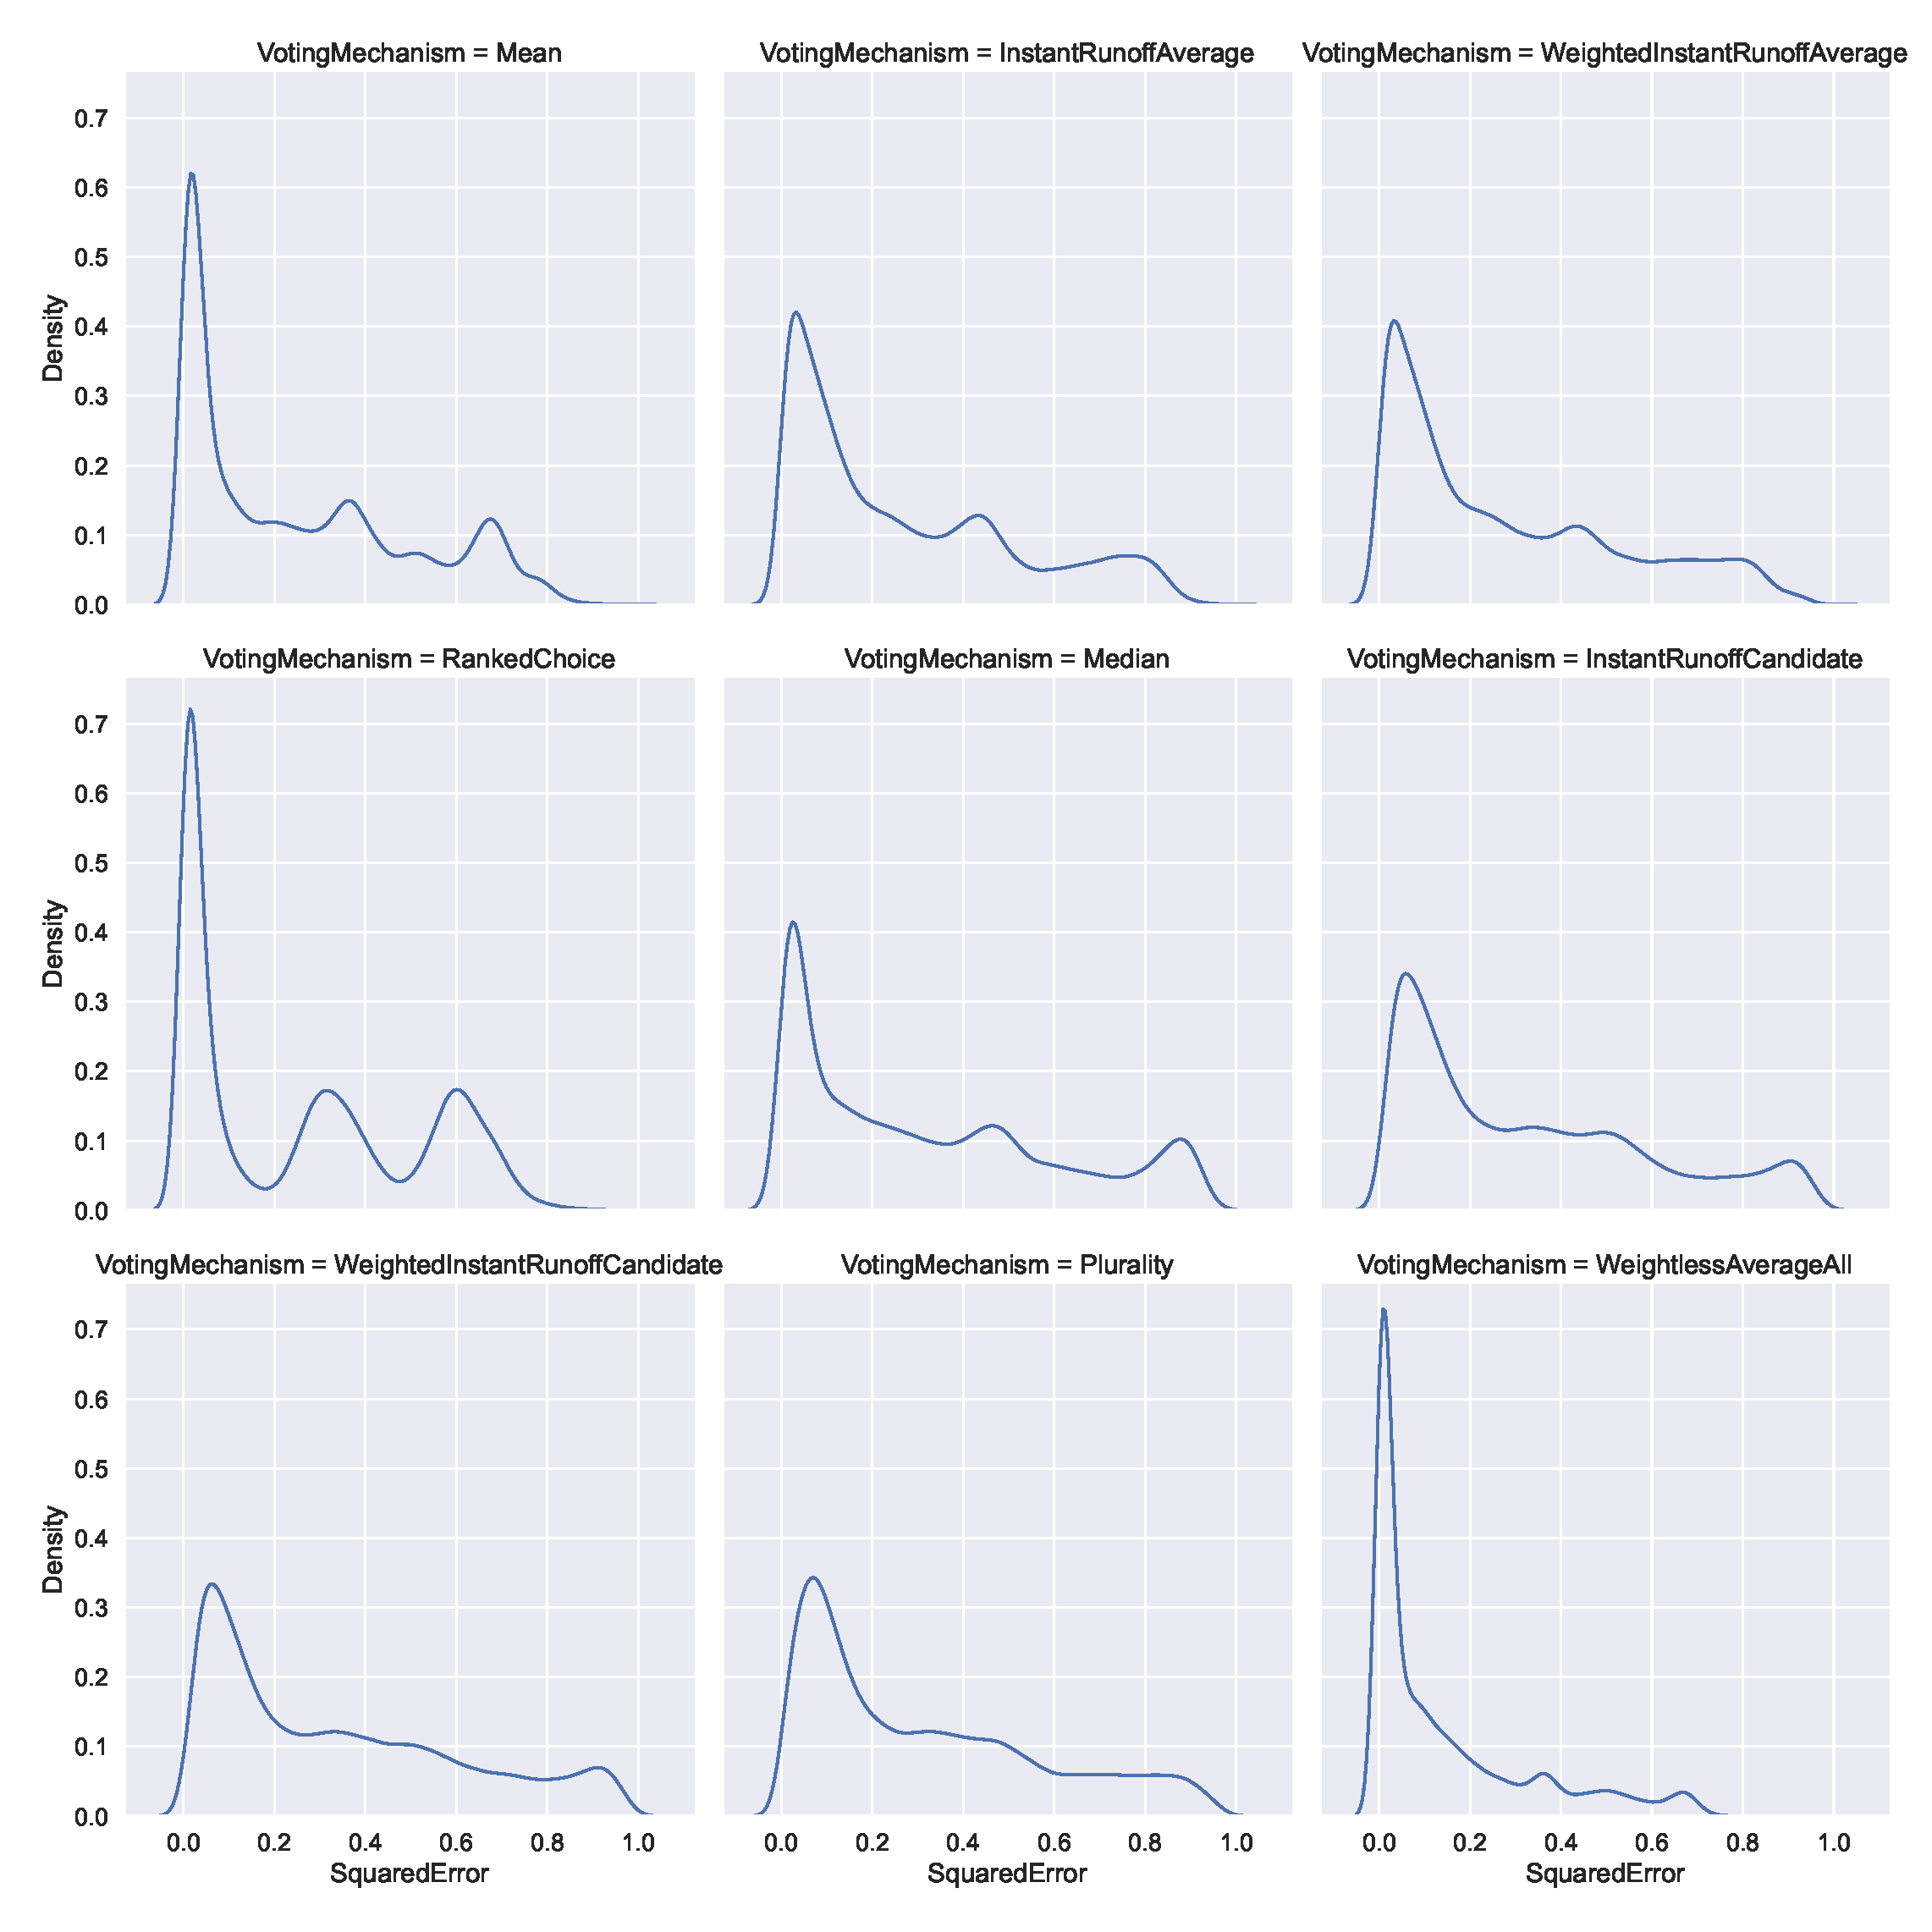
\includegraphics[
        width=\textwidth,
        height=\dimexpr
        \textheight - 2 % Could also be .9\textheight
        \baselineskip,
        keepaspectratio]
    {./content/figures/voting_mechanisms_distribution}
    \caption{The distribution of squared error by voting mechanism}
    \label{fig:voting_mechanisms_distribution}
\end{figure}

%    \include{vita}  % FIXME: I don't think I actually need this unless I'm a doctorate.
    %}}}
\end{document}
